%auto-ignore
%      this ensures the arxiv doesn't try to start TeXing here.
%!TEX root = super_lattice_models_draft.tex
%      prev line helps TeXShop do the right thing



%%%%%%%%%%%%%%%%%%%%%%%
\section{Super pivotal state sums and tensor networks} \label{state_sums}
%%%%%%%%%%%%%%%%%%%%%%%

\dave{Note to self: look at \cite{beliakova1998}.}

In this section we write down a Turaev-Viro-Barrett-Westbury (TVBW) state sum \cite{Turaev1992,Barrett1996}
for the super pivotal fusion categories, 
and a tensor network for the ground state wave function of the Hamiltonian constructed in Section \ref{Super_pivotal_Hamiltonian}.
%\eqref{ham}.
%Very closely related 
Related 
%\kw{very closely related, or just related?
%I could not tell after a quick look at the paper.}
work was presented in~\cite{bhardwaj2016}, 
see also \cite{Bultinck2017, upcoming-paper?}.
\kw{fix citation}
We first review the TVBW construction for bosonic spherical fusion categories. 
We then show how to write the state-sum as a tensor contraction on a tensor 
network.
Next we detail the modifications needed for the fermionic versions of the state sum and tensor network.
%which allows us to extend the state-sum to the super-pivotal case with only minor modifications.
Lastly we use the state sum to write down an explicit wave function for the ground ground state of \eqref{ham}.

%We first give a lightning review of the TVBW state sum construction, via the cut-and-glue formalism.
%Since much is known about TVBW state sums, 
%we present the state sum from a slightly different perspective than usual,
%so that the fermionic version of the state sum can be written in essentially the same way.

%We view the state sum as a composition of linear maps from finite dimensional tensor product spaces, starting with with the ``vacuum" $\cc$. 
%\kw{Still not convinced that this is a valid way to look at it; maybe I will be convinced when I read further.}
%This composition of linear maps can be interpreted as a tensor network, 
%which we investigate in the subsequent sections.

%The starting point is a list of data:
%\dave{Is pivotal and spherical the same thing?
%I remember getting quite confused about this in a Muger paper.} %\ethan{I think yes}
%\begin{itemize}
%\item a spherical fusion category $\mcc$,
%\item an oriented 3-manifold $M$,
%\item and a cell decomposition with oriented 1-cells and transversally orientated 2-cells (equivalently, the boundary of the 2-cells has an orientation)
%\end{itemize} 
%from which one defines a partition function $Z(M)$. 

%To define these linear maps, we will follow a `cut-and-glue' approach.
%Schematically, this proceeds by cutting up the manifold on which we want to evaluate the state sum into many parts. 
%We assign vector spaces to each of the cut-up pieces and then 
%construct the state sum by gluing these pieces back together with linear maps that are given by performing tensor contractions.
%In order for our formalism to be amenable to fermionic modifications, we will need to carry out a 
%standardization procedure of the cell decomposition of $M$, in much the same way that we 
%performed the standardization procedure to define the lattice Hamiltonian. 
%This is the issue to which we first turn. 
%Much of the following section is notational; 
%readers are invited to familiarize themselves with Figure~\ref{NotationStateSum}
%and \eqref{attaching_region}-\eqref{tensor_space}, 
%and continue with the next subsection. 

%\subsection{Cell and a Handle decomposition}
%\ethan{since this is just a paragraph, I don't think it needs its own subsection}
%\kw{Perhaps discussion relating handle decompositions to cell decompositions should go first.
%It will be convenient for us to be able to describe things in terms of both 
%a handle decomposition and also the corresponding cell decomposition.}

\medskip

Before we begin, we need to establish some terminology regarding cell and handle decompositions. 
Recall that a handle decomposition for a 
3-manifold $M$ is built from a series of $k$-handles, with $k=0,1,2,3$, each of which is identified with $D^k\times D^{3-k}$. 
Handle decompositions can be obtained from cell decompositions by thickening each $k$-cell into a $k$-handle.
Conversely, each handle decomposition determines a cell decomposition by taking the cores of the handles.
(See Section \ref{standardized_handles} for more details.)
%Each $k$-handle is obtained from a $k$-cell by ``fattening'' the $k$-cell in the manner described 
%in Section \ref{standardized_handles}.
We will often refer to a $k$-cell and its associated $k$-handle with the same letter, since
it will be convenient for us to be able to describe things in terms of both handle decompositions 
and their corresponding cell decompositions. 
We call $S^{k-1} \times D^{3-k}$ the attaching region (or attaching boundary) of the $k$-handle,
and $D^k\times S^{3-k-1}$ the non-attaching boundary.
%The attaching region of a $k$-handle is $S^{k-1} \times D^{3-k}$,
The attaching map of a $k$-handle is a homeomorphism from the attaching region to 
a submanifold of the boundary of the union of the lower-dimensional handles.
The topology of $M$ is encoded by the various attaching maps.
\davex{Maybe draw a figure showing 0-, 1-, 2- and 3-cells and the corresponding 0- 1-, 2- and 3-handles.
\ref{cell_and_handle_decomp}}
\begin{figure}
\begin{align}
%\text{a figure} 
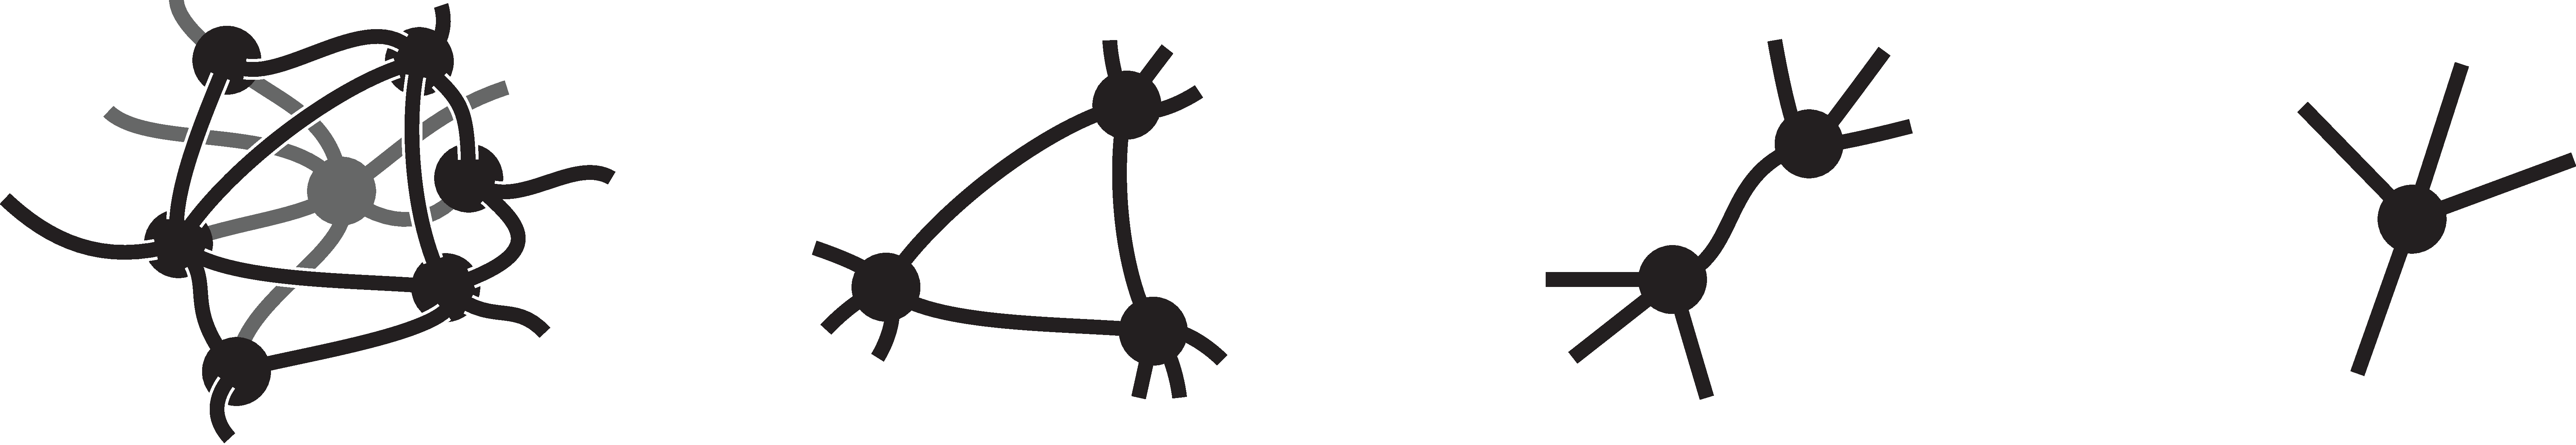
\includegraphics[scale = 0.1]{CellDecompFig.pdf}
\end{align}
\caption{
\label{cell_and_handle_decomp}
\davex{Figure done quickly, had to leave during making.
Should add something about handle decompositions.}
Here we show part of a cell decomposition and its associated handle decomposition. 
An example of each k-cell.
On the left we have a 3-cell given by the volume inside the adjacent 0-, 1-, and 2-cells. 
Second from the left we have a 2-cell and its adjacent 0- and 1-cells. 
Second from the right have a 1-cell and its adjacent 0-cells.
On the right we have a 0-cell.
}
\end{figure}
%is built into the attaching regions where different handles are connected, each of which is homeomorphic to $S^k \times D^{n-k}$.
%We are interested in 3-manifolds,
%and hence the attaching regions between between the $(k+1)-$ and $k$-handles are given by
%$S^2 \times D^0$ (3-handles to 2-handles), $S^1 \times D^1$ (2-handles to 1-handles), and $S^{0} \times D^2$ (1-handles to 0-handles).
%%KW k-handles attach to the boundary of the 0, 1, ... k-1 handles, not just the k-1-handles
%Although not necessary, we assume the cell decomposition of $M$ is dual to a triangulation for ease of notation.
%The standardization procedure is similar to the pitchforkization procedure defined in \eqref{pitchfork_basis} and surrounding text.


\kw{to do: restore description on relation of cell decomps to handle decomps; also establish conventions for manifolds
with boundary}


\begin{comment}
\ethan{this is Kevin's second outline, commented it out since it was cluttering up things}
\subsection{Outline of proposed reorganization (KW)}	%%%%%%%%%%%%%%%%%%%%%%%%%%%

\kw{My hope was that the notation and order of presentation below would be in close-to-final form, but currently
I'm falling short of that goal.}

\kw{Still in progress.}

\medskip

Outline:
\begin{itemize}
\item Review bosonic state sum, on general cell decomp
\item How to turn this into a tensor network
\item Discuss ways to standardize (generic cell decomp (dual to triangulation), global ordering (which has
some disadvantages in our intended application)
\end{itemize}

\kwsep
\end{comment}


%%%%%%%%%%%%%%%%%%%%
\subsection{Bosonic TVBW state sum}
%%%%%%%%%%%%%%%%%%%%

\subsubsection{Definition of the state sum}


Our first task is to describe the TVBW (bosonic) state sum.
The original references are \cite{Turaev1992,Barrett1996}.
We will use the form for a general cell/handle decomposition, as described in \cite{Walker2006}.

Let $M$ be a closed oriented 3-manifold equipped with a handle decomposition $\mch$.
Choose auxiliary orientations of the 1- and 2-cells of the cell decomposition corresponding to $\mch$.
Let $\mch_i$ denote the set of $i$-handles ($i = 0,1,2,3$).
The state sum has the form
\be \label{bos_tv_sum}
	Z(M) = \sum_{\beta\in\mcl(\mch)}
		\prod_{c\in\mch_3} \mcd^{-2}
		\prod_{f\in\mch_2} d(f, \beta)
		\prod_{e\in\mch_1} \widetilde\Theta(e, \beta)^{-1}
		\prod_{v\in\mch_0} \text{Link}(v, \beta) .
\ee
The next few paragraphs define the notation used in \eqref{bos_tv_sum}.

%%%%%%%%%%%%%%%%%%%%
% old figures %%%%%%%%%%%%%
\begin{comment}
\begin{figure}
\begin{center}
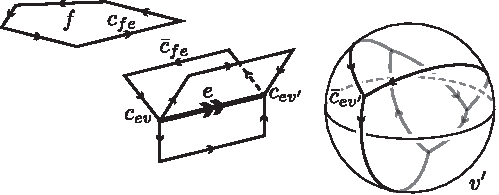
\includegraphics{NotationStateSum.pdf}
\caption{\label{NotationStateSum}
Notation used in this section. 
%The cells can be used to label the weights that determine the partition function.
In the figure we have labeled a 2-cell (face) by $f$, a 1-cell (edge) by $e$, and a 0-cell (vertex) by $v$. 
We assume a cell decomposition that is dual to a triangulation, so that each 1-cell is adjacent to three 2-cells and two 0-cells, 
and each 0-cell is adjacent to four 1-cells. 
The boundary of each 2-cell $f$ possesses an orientation (left). 
The 1-cells are also oriented, with the orientation of the edge $e$ in the figure indicted by the double arrow (center). 
The oriented boundary edge of the face $f$ that neighbors the edge $e$ is labeled $c_{fe}$ (left), 
and the opposing edge that is glued to $c_{fe}$ is labelled by $\bar{c}_{fe}$. 
The trivalent junctions occurring at either end of the edge are denoted $c_{ev}$ and 
$c_{ev'}$ (center).
A small $S^2$ surrounding a 0-cell $v'$ intersects six 2-cells in six oriented lines, which 
meet at four trivalent junctions $\bar{c}_{ev'}$ (right). 
\dave{Is this figure still useful for anything?}
\ethan{I guess not. Makes me sad, though} 
\kw{I think the figure is still useful; eventually we restrict our attention to this sort of cell decomposition.}
\kw{Might want to include two figures, or a 2-part figure, that illustrates (1) arbitrary cell decompositions, and 
(2) generic cell decompositions}
}
\end{center}
\end{figure}

\begin{figure}
\begin{center}
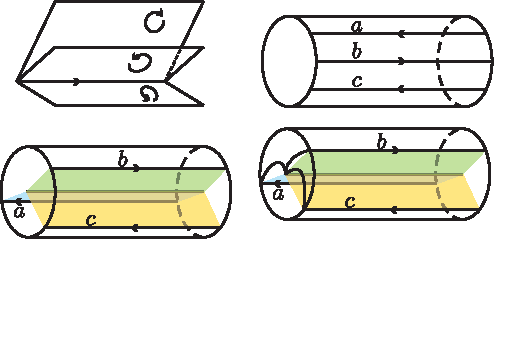
\includegraphics{Onehandle_smaller.pdf}
\caption{\label{One_handle}
Various pictures relating to our presentation of the 1-handles. In the top left picture, we show
three 2-cells which terminate on a given 1-cell, with the orientations of the 2-cells shown as curly arrows. 
In the top right picture we show a 1-handle with its three marked edges and their orientations shown. 
In the bottom left we have the same picture as in the top right, but with the intersection of the 2-cells 
with the 1-handle shaded in color. In the bottom right picture, we show the same picture as in the bottom left, but this time with the vertices standardized via our pitchforkization procedure. 
\ethan{may need to update the bottom right guy, although I'm in favor of keeping the pitchforkization standardization procedure}
}
\end{center}
\end{figure}
\end{comment}
%%%%%%%%%%%%%%%%%%%
%%%%%%%%%%%%%%%%%%%%


\begin{figure}
\begin{center} 
\begin{align}
\nonumber
\TwoHandleToGraph
\end{align}
\caption{\label{TwoHandleToGraph}
\davex{Note to self: 
Just draw attaching graph on 2-handle (no 2-cell). 
Remove all 2-cells.}
\davex{Is this roughly what we were thinking? (probably need to come back to this and get the coloring right etc. )
Will have to modify caption once figure is decided on.}
%\davex{
%Do you guys think a figure of this type would be helpful to show how a 2-cell determines the graphs on the adjacent 0- and 1-handles?
%If so I'll make it look better, if we're going to scrap it, then I won't bother.}
%\ethan{this figure is awesome}
%\ethan{but, I don't understand the reason for including the left picture (other than that it looks cool)}
%\davex{To show how the 2-cell determines the attaching core of a 2-handle.}
%\kw{I also find the left fig confusing}
%\davex{Removed the left figure. Also going to remove the associated comments.}
A triangular 2-cell and its adjacent 0- and 1- and 2- handles. 
The oriented 2-cell determines part of the graphs on each 0-, 1- and 2-handle. 
On the left we show the graph found at the intersection of the 2-cell with the 2-handle.
On the right we show the part of the graphs on each 0- and 1-handle determined by the 2-cell.
We have omitted the attachment regions on the 1- and 0-handles that do not intersect the shaded 2-cell.}
\end{center} 
\end{figure} 

We use the 2-cell orientations to define an oriented graph (unlabeled string net) on the boundary of each 0-, 1- and 2-handle,
as shown in Figure \ref{TwoHandleToGraph}.
% \ref{NotationStateSum}.
%\dave{I don't think we should recycle that figure here. 
%I think we need a figure that shows how each 2-cell orients a part of the 2-, 1- and 0-cells.
%I'll try to think of a reasonable figure to draw.}
String-net graphs are assigned to the $k$-handles as follows:
\kw{KW to-do: maybe draw another fig for this}
\begin{itemize}
\item On 2-handles, the graph is a single loop along the core of the attaching annulus of a 2-handle.
The orientation of the loop is determined by the orientation of the 2-cell. 
%For a 2-cell 
%$f$, this is shown in the top left of Figure \ref{NotationStateSum}. \ethan{may wan to remove the $c_{fe}$ stuff from the figure}
\item On 1-handles, the graph is a generalized $\Theta$ graph, which we will call a $\widetilde\Theta$ graph.
The graph has one edge for each 2-handle adjacent to the 1-handle.
The middle part of each edge of the graph corresponds to where the cores of the 2-handles meet the boundary of the 1-handle.
The two vertices of the graph are on the two attaching disks of the 1-handle.
The edges are oriented opposite to the orientations used in the 2-handle loops above.
\item On each 0-handle, the graph is determined by the pattern of 2- and 1-handles adjacent to the 0-handle.
The graph has one edge for each adjacent 2-handle and one vertex for each adjacent 1-handle.
The orientations of the edges are opposite to the orientations of the 2-handle loops.
We denote this graph $\text{Link}(v)$.
%Each edge of the graph corresponds to the lines where the 2-handles meet the boundary of the 1-handle, which is shown in the bottom-left picture of Figure \ref{One_handle}. 
%The graph associated to the 1-handle has two vertices, which are located on the two attaching disks of the 1-handle (which are the disks where the 1-handle is attached the the 0-handles it connects).  
%The edges on the 1-handle are oriented oppositely to the orientations of the respective 2-handle loops.
%For example, we can use the 2-handle orientations shown in the top left picture of Figure \ref{One_handle}
%to determine the orientations of the edges marked $a,b,c$ in the remaining pictures. 
%\item On each 0-handle, the graph is a string-net on a sphere determined by the pattern of 2- and 1-handles adjacent to the 0-handle.
%The graph has one edge for the lines where each 2-handle adjacent to the 0-handle intersect it;
%these lines intersect at vertices at the location where each adjacent 1-handle meets the 0-handle. 
%The orientations of the edges in this graph are drawn opposite to the orientations of the 2-handle loops.
%We denote this graph $\text{Link}(v)$.
%For a 0-handle with four adjacent 1-handles, an example of a graph determined by such 
%a procedure is shown as the rightmost picture in Figure \ref{NotationStateSum}. 
%\ethan{I might be in favor of Tet (even though we are now not working with something dual to a triangulation)}
\end{itemize}

\begin{figure}
\centering
\begin{align}
\nonumber
\CellDecompNearOneHandle \quad \quad \quad \quad \quad \OneHandlePrime 
\end{align}
\caption{\label{OneHandlePrime}
On the left, we have an illustration of four 2-cells meeting a 1-cell.
For clarity we have put a small gap between the 1-cell and the four 2-cells.
On the right we have the corresponding 1-handle and a particular labeling. 
We have denoted the corresponding attaching disks by `i' for initial, and `t' for terminal. 
}
\end{figure}

Recall that we have an orientation of each 1-cell.
This allows us to distinguish an ``initial" and ``terminal" attaching disk for each 1-handle; see Figure \ref{OneHandlePrime}.
On the initial disk we see a graph with a single vertex in the interior of the disk and $k$ edges connecting the central vertex
to the boundary of the disk (where $k$ is the number of 2-handles which cross the 1-handle).
For each labeling $\ell$ of these edges by simple objects in $\sob(\mcc)$, we have an associated vector space $V(\ell)$.
For example, in the case of Figure \ref{OneHandlePrime} the vector space is isomorphic to $V^{ab^*c^*d}$.
Let $B(\ell)$ be some chosen basis of this vector space.
For each 1-handle $e$ define $B(e)$ to be the union over all labelings $\ell$ of $B(\ell)$,
and also define $V(e)$ to be the direct sum of all the vector spaces $V(\ell)$.

%Recall that we have an orientation of each 1-cell.
%This allows us to distinguish an ``initial" and ``terminal" attaching disk for each 1-handle.
%For example, for the 1-handle drawn in Figure \ref{One_handle}\dave{Lets modify the figure.}, the left end of the 1-handle would 
%host the initial attaching disk, while the right end of the 1-handle would host the terminal 
%attaching disk. 
%On the initial disk we see a graph with a single vertex in the interior of the disk and $k$ edges connecting the central vertex
%to the boundary of the disk ($k$ is the number of 2-handles adjacent to the 1-handle).
%For each labeling $\ell$ 
%\ethan{changed $b$ to $\ell$ since we use $b$ for simple objects all the time}
%\dave{Good idea.}
% of these edges by simple objects in $\sob(\mcc)$, we have an associated vector space $V(\ell)$.
% For example, in the case of fig xxxx the vector space is isomorphic to $V^{ab^*c^*d}$
% \dave{I'm guessing this was meant to be a one-hadnle example with 4 neighbouring 2-cells.}.
%For example, in the case of Figure \ref{One_handle} the vector space is isomorphic to $V^{a^*bc^*}$.
%Let $B(\ell)$ be some chosen basis of this vector space.
%For each 1-handle $e$ define $B(e)$ to be the union over all labelings $b$ of $B(\ell)$,
%and also define $V(e)$ to be the direct sum of all the vector spaces $V(\ell)$.

We define the set of all labelings $\mcl(\mch)$ to be the product over all 1-handles $e$ of the basis sets $B(e)$.
In other words, we choose (independently, without any compatibility constraints) a labeling by simple objects of the edges of each initial
disk graph, then choose a basis vector for each associated vector space.

We also associate a vector space $V^*(\ell)$ to the terminal disk of each labeled 1-handle.
%\dave{Should we use a different star here? 
%Since it is somewhat different than the two stars we defined in the definition section.
%Or maybe we should just use $V^i(e)$ and $V^t(e)$ for initial and terminal vector spaces. 
%Then use $(V^i(e))^*$ and $(V^t(e))^*$ for their respective duals as defined by the `standard' reflection pairing (input vector spaces to $\text{Link}(v)$.)
%}
%\dave{I retract this comment.}
In the example, this is isomorphic to $V^{d^*cba^*}$.
%In the example, this is isomorphic to $(V^{a^*bc^*})^*$.
%We also define $V^*(e)$ to be the direct sum (over all labelings $b$) of $V^*(\ell)$.
There is a nondegenerate bilinear pairing between $V(\ell)$ and $V^*(\ell)$, 
given by evaluating the labeled string net on the boundary of the 1-handle (which is a 2-sphere).
%(This is closely related to the pairing \eqref{reflection_pairing_defn}.)
%found by applying the standard bilinear pairing \eqref{reflection_pairing_defn} after a rigid translation through the 1-handle.
%\eqref{reflection_pairing_defn} and 
%graphically looks like a banana. % :--)
%\ethan{we should probably change $\mcb$ to $\Theta$ or the other way around to make notation consistent}
%\dave{Or should we change $\mcb$ to $\widetilde{\Theta}$ and save $\Theta$ for trivalent junctions?}
%\dave{Need to consider whether we put the pivots on the 1-handles or the 0-handles.}
%\ethan{whether we want a back reference to $\mcb$ is tbd}
We will choose a basis of $V^*(\ell)$ such that the pairing matrix is diagonal.
(It is sometimes convenient to not insist that the diagonal entries be $\delta_{ij}$.)
%As with $\mcb$, it is sometimes convenient to not insist that the diagonal entries be $\delta_{ij}$.
We also define $V^*(e)$ to be the direct sum (over all labelings $\ell$) of $V^*(\ell)$.

We are now ready to define the weights appearing in the state-sum $Z(M)$. 
Let $\beta\in\mcl(\mch)$ and let $f$ be a 2-handle.
The labeling $\beta$ associates a simple object to each intersection of $f$ with a 1-handle.
If these simple objects are not all the same, we define $d(f, \beta) = 0$.
If they are all equal to the same simple object $a\in\sob(\mcc)$, we define the weight $d(f, \beta)$
appearing in \eqref{bos_tv_sum} by $d(f,\beta) = d_a$.

Let $e$ be a 1-handle.
The labeling $\beta$ associates a basis vector $\mu$ to the initial disk of $e$.
Define $\widetilde\Theta(e, \beta)$ to be the value of the bilinear pairing evaluated on $\mu^*$ and $\mu$.
%\dave{I'm guessing with this convention we have cut the 1-handle between the two 0-handles. 
%Otherwise if we cut at the ends near the 0-handles we need $\widetilde{\Theta}  \ra \frac{\widetilde{\Theta}\widetilde{\Theta}  }{ \widetilde{\Theta} } $ in $\widetilde\theta$ in $Z(M)$.
%Two standard ones coming from the attaching disks of the 1-handle, and one non-standard one that depends on the 1-handle itself (e.g., could have a pivot).
%Is that correct? Should we mention this?
%}
Diagrammatically, $\widetilde\Theta(e, \beta)$ is found by connecting the open strings in $V(\ell)$ to their dual counterparts in $V^*(\ell)$ and evaluating 
the resulting diagram.
Continuing with our example in Figure \ref{OneHandlePrime}, 
%%KW 2-handles don't get directly labeled
%if $e$ has four adjacent 2-handles labeled by $a,b,c,d$ with the orientations of Figure \ref{OneHandlePrime} so that $\mu \in V^{ab^*c^*d}$, then 
we have 
\be \label{four_banana}
\widetilde \Theta (e, \beta) =  \Bananafourmu.
\ee
%\ethan{need to change $\eta_i$ in the fig to $\mu^*$ and $\mu$}
%\dave{done}

\begin{figure}
\centering
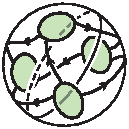
\includegraphics{TetSphereColored.pdf}
\caption{ \label{TetSphere_Fig} 
An example of the surface of a 0-handle on which four 1-handles are attached to. 
The attaching regions for the 1-handles are marked in green, and those for the 
2-handles are shown as purple strips. The coloring $\beta$ assigns 
objects to the purple strips and fusion space basis vectors to the green regions.
\dave{may need to add orientations of 1-handles}
}
\end{figure}

Let $v$ be a 0-handle.
The labeling $\beta$ determines a labeling of the graph $\text{Link}(v)$ as follows.
Near each vertex of $\text{Link}(v)$ we place the basis element $\mu^* \in V^*(e)$ (or $\mu \in V(e)$) assigned by $\beta$ to the 
corresponding 1-handle if $v$ is attached to the initial (terminal) end of the 1-handle.
%\footnote{The dual spaces here are determined by the bilinear pairing of \eqref{reflection_pairing_defn}.}
%\dave{I think it should be $\mu^* \in V(e)^*$ and $\mu \in (V^*(e))^*$.}
%\ethan{to make it consistent with our earlier writing of the section, I think yes. I interchanged them.}
If these vertex labels are incompatible along edges of $\text{Link}(v)$, we define $\text{Link}(v, \beta) = 0$.
If they are all compatible then we define $\text{Link}(v, \beta)$ to be the evaluation of the resulting labeled graph (string net).
%\ethan{The evaluation is zero if they aren't compatible, so we can just say it's the evaluation and leave it at that.}
%\kw{I would say the evaluation is not defined if the labels do not match.}
For cell decompositions dual to a triangulation, 
the labeled graph is a tetrahedral string net on a sphere.
This is illustrated in Figure \ref{TetSphere_Fig}, which shows an example 0-handle on which 
four 1-handles terminate. The attaching regions for the 1-handles are marked in green, and those 
for the two-handles are marked in purple. $\beta$ assigns string-net labels to the purple strips and 
basis elements $\mu$ to the green regions, with ${\rm Link}(v,\beta)$ being computed by evaluating the resulting graph on the sphere. 

This completes the definition of the state sum.

\medskip

It follows from Section 8.2 of \cite{Walker2006} that the state sum computes $Z(M)$, independently of the choice of handle decomposition
and choice of orientations of 1- and 2-cells.

\medskip

If $M$ has non-empty boundary,
we choose the handle decomposition to have the form shown in Figure xxx \kw{fix ref} near the boundary.
In terms of cell decompositions, we choose a cell decomposition such that $\bd M$ lies in the 2-skeleton, rather
than a cell decomposition such $\bd M$ is transverse to the cells.

The 0- and 1-cells on $\bd M$ will do double duty as the underlying graph of a string net on $\bd M$.
Choose an orientation of each 1-cell on $\bd M$.
(This is analogous to choosing an orientation of the boundary of a 2-cell in the interior of $M$.)
Choose a labeling of these oriented edges by simple objects in $\sob(\mcc)$.
For each vertex (0-cell) on $\bd M$, choose an element of the appropriate disk vector space
(e.g.\ $V^{ab}_c$ in Figure xxxx).

We now have a labeled string net $g$ on $\bd M$.
The state sum will evaluate the path integral $Z(M)(g)$ 
(i.e.\ the path integral of $M$ with boundary condition given by $g$).
The labelings and weights are defined as before, except that some of the labels are already determined by the string net $g$ on the boundary.

%%KW accidentally rewrote this above; not sure which version is better.
%We also choose a string net on $\bd M$ compatible with the handle decomposition (a labeled edge
%for each 1-handle along $\bd M$, and a labeled vertex for each 0-handle along $\bd M$).
%We modify the label set $\mcl(\mch)$ to be fixed for strands on $\bd M$ and varying for interior labels.
%The modified state sum assigns a number to each fixed boundary string net.
%This can be interpreted as a linear function $A(\bd M)\to\cc$ (i.e., a wavefunction).
%%which gives us a wavefunction, i.e. linear function $A(\bd M)\to\cc$.

%\dave{Maybe think about reference to wavefunction.}


%%%%%%%%%%%%%%%%%%%%%%%%%
\subsubsection{The state sum as a tensor network}
%%%%%%%%%%%%%%%%%%%%%%%%%

Our goal in this subsection is to reinterpret \eqref{bos_tv_sum} as a tensor network.
We will first discuss that case when $M$ is closed, then consider the case when $\bd M$ is non-empty.
%\ethan{replaced ``regularization'' with ``standardization'' since regularization has a different physics meaning}
%\dave{Definitely a good idea.}

\medskip

If we (temporarily) ignore the factors of $d(f, \beta)$ and $\mcd^{-2}$ in \eqref{bos_tv_sum}, 
it is easily seen to compute the contraction of a tensor network.
%it is easy to see that it computes the tensor contraction of a tensor network.
The underlying graph of the tensor network is the union of 0- and 1-cells of the cell decomposition.
The vector space associated to each edge $e$ is $V(e)$ as defined above.
The matrix elements of the tensor associated to a 0-cell $v$ are the numbers $\text{Link}(v, \beta)$ defined above.
The factors of $\widetilde\Theta(e, \beta)^{-1}$ arise from the pairing of dual tensor indices.
%\kw{Say more about this?}
%\kw{remark about dual spaces here??}
%\dave{What did you have in mind?}

To incorporate the factors of $d(f, \beta)$ and $\mcd^{-2}$, we make some ad hoc choices.
We consider ``dressed" 
%\kw{Is this the usual meaning of ``dressed"?  If so, great.}
%\dave{If you are happy with thinking of $d(f, \beta)$ and $\mcd^{-2}$ as being clothes for $\text{Link}(v,\beta)$ then, yes. 
%But more seriously. I don't think it has a super established meaning, and don't think it would raise eyebrows. 
%I think in a lot of the physics literature it appears as ``dressing'' domain walls.
%It's sometimes used to avoid writing down an explicit Hamiltonian and only talking about the physics of a hypothetical Hamiltonian. 
%}
0-handle weights that tack on the factors of $d(f,\beta)$ and $\mcd^{-2}$.
For each 2-handle $f$ we choose an adjacent 0-handle $v_f$.
For a 0-handle $v$ we modify the associated weight ${\text{Link}}(v,\beta)$ by multiplying factors of $d(f,\beta)$ for each 2-handle $f$ such that $v = v_f$.
Similarly, for each 3-handle we choose an adjacent 0-handle and multiply the associated weight by $\mcd^{-2}$.
Denoting the modified 0-handle weights by $\widetilde{\rm Link}(v,\beta)$, 
%we construct the vertex tensor 
%Denoting the modified 0-handle weights by $\widetilde{\rm Link}(v,\beta)$, we construct the vertex tensor 
%\be 
%	T_v = \sum_{w_v } \widetilde{\text{Link}}(v,w_v) w_v,
%\ee
%where the sum runs over orthogonal basis vectors for the vector space associated to the attaching disks of $\text{Link}(v)$ (the vector space for each attaching disk on $\text{Link}(v)$ is dual to the vector space associated to the initial/terminal attaching disks of the adjacent 1-handles).
%for the vertex Hilbert space $\mch(v)$. 
%\kw{I think we need to say this a little differently; we don't have any inner products defined,
%so we need to carefully distinguish between spaces and dual spaces.}
%\dave{Changed it to the above.
%}
%\kw{One of the $w_v$ needs to be in a dual space; otherwise it scales incorrectly.  Maybe I'll edit it more later.}
%\dave{I can't argue with that. 
%I think my vote would be to let $w_v$ be the tensor product of the vector spaces associated with the ends of the 1-handles 
%(i.e., if a 1-handle $e$ is emanating from $v$ then one of the tensor factors would be living in $V(e)$).
%Then write $\widetilde{\text{Link}}(v,w_v^*) w_v$.
%}
%\kw{Why not just define $T_v$ as follows? ...}
%\dave{Works for me.}
we define the 0-handle tensors $T_v$ as follows.
Let $e_1, \ldots, e_k$ be the 1-handles adjacent to the 0-handle $v$.
Let 
\begin{align}
\label{0_handleVectorspaces}
V_i = \begin{cases}
V(e_i) & \text{if $v$ is adjacent to the terminal end of $e_i$}\\
V^*(e_i) & \text{ if $v$ is adjacent to the initial end of $e_i$}.\\
\end{cases}
\end{align}
%Let $V_i$ be either $V(e_i)$ (if $v$ is adjacent to the terminal end of $e_i$)
%or $V^*(e_i)$ (if $v$ is adjacent to the initial end of $e_i$).
We define
\be
	T_v \in V^*_1\tp\cdots\tp V^*_k
\ee
by
\be
\label{vertex_tensor}
	T_v(w_1\tp\cdots\tp w_k) = \widetilde{\text{Link}}(v, w_1\tp\cdots\tp w_k),
\ee
where $w_i\in V_i$.
In other words, $T_v$ evaluates the link graph with labels determined by $w_1,\ldots,w_k$ and multiplied by the factors of $d(f,\beta)$ and $\mcd^{-2}$ as described above.
%\kw{... end ``as follows"}
%\dave{Is this necessary?}
%\ethan{It was intended to be my guess to what Kevin's dual spaces comment meant. Might have missed the mark though, and it might still be confusing.}
To obtain the partition function, we trace out the tensor product of all the 0-handle tensors constructed in this way.
Because the vector space associated to the region on a $0$-handle attached to the 
terminal end of a 1-handle $e$ is dual to the vector space associated to the corresponding region on the 
0-handle attached to the initial end of $e$, there are precisely as many dual vectors as vectors in the tensor product, and 
contracting each vector with its associated dual vector computes the complex number $Z(M)$. 
That is, we have 
%\ethan{I think we need something like this. If you guys don't like tTr then we can use an appropriately normalized $\Theta$ instead}
%\dave{I like ${\rm tTr}$ for now.
%We do need to define it though.}
%\kw{Maybe $\text{tc}$ for tensor contraction?}
%\dave{I think Gu-Levin-Wen used ${\rm tTr}$ (in a similar context), which is one reason to stick with it. 
%Although would have to check if it's been used much since.
%Sometimes people use $C( ....) $ for contraction, or even $\mcc(...)$. 
%Both of those would probably be a nuisance in this paper though. 
%$tc$ for tensor contract is nice, my only reservation is that there is probably a few other notations that have been established. 
%}
%\dave{It's kind of like $\text{eval}^{-1}$. 
%Is there a standard tensor category name for that?}
%\kw{If tTr is well established, then fine.  Otherwise maybe a simple tr would do.
%I think tr is often used in this generalized sense in math papers.}
%\dave{I talked to one friend, he didn't think there was any well established notation for this. }
\be Z(M) = \tr \left(\bigotimes_{v\in \mch_0} T_v\right),\ee
where the trace $\tr$ denotes the tensor contraction.
%%KW not sure why this remark is necessary; also ``normalized" doesn't seem like the right word.
%It is normalized so that a factor of $\widetilde{\Theta}^{-1}$ is introduced if the labels on each side of the 1-cell are dual to one another (with respect to the bilinear pairing) and is zero otherwise.\footnote{Alternatively we could use the standard pairing but then we would have to modify our vertex tensors by $T_v(w_1\tp\cdots\tp w_k) \ra T_v(w_1\tp\cdots\tp w_k) \widetilde{\Theta}(e_1,w_1)^{-1} \cdots \widetilde{\Theta}(e_k,w_k)^{-1}$  }
%\dave{May want to be more explicit.}
%\kw{This may have already been discussed above}
%\dave{I'll keep an eye out.}
It is easy to see that this tensor network gives the same state sum as \eqref{bos_tv_sum} and 
is independent of the way we assign factors of $d(f,\beta)$ and $\mcd^{-2}$ to the 
vertex tensors. 

\medskip

%In the case where $\partial M \neq \emptyset$, the Hilbert space associated 
%with the tensor product of the 0-cell tensors admits a decomposition $\mch^*_{bulk} \tp \mch_{bulk} \tp \mch(\bd M)$, where 
%the Hilbert spaces of the degrees of freedom on $\partial M$ lack dual tensor factors appearing in the tensor product. 
%The partition function is still performed by contracting, which contracts out the tensor factors in $\mch^*_{bulk} \tp \mch_{bulk}$ but leaves those in $\mch(\partial M)$ uncontracted, producing a wavefunction supported on $\mch(\partial M)$ (that is, a map $A(\partial M) \ra \cc$).
%\kw{This is basically correct, but let's work on the phrasing.}

%\dave{This version looks good to me.
%I'll come back to this}
In the case where $\partial M \neq \emptyset$, we define the 0-handle tensors $T_v$ as before,
but in this case some of the legs of the tensors are unpaired (not contracted).
Specifically, there is one unpaired leg for each 0-cell on $\bd M$.
If $W_1, \ldots, W_n$ are the vector spaces associated to the boundary 0-cells, we have
\be \label{trace_pM_nonempty}
	Z(M) = \tr \left( \bigotimes_{v\in \mch_0} T_v \right) \in W_1^*\tp\cdots\tp W_n^* .
\ee
Each string net on $\bd M$ (i.e. each labeling of 0- and 1-cells as described above)
determines an element of $W_1\tp\cdots\tp W_n$ (the vertex labels).
By evaluating \eqref{trace_pM_nonempty} on this element we obtain the amplitude of the wave function for the string net.
\kw{chaged ``value" to ``amplitude" -- look OK?}
%\kw{rephrased the end of this paragraph}
%\ethan{I like the new sentence} 
%\davex{Maybe change `value' to `amplitude': something like ``...we obtain the amplitude for the wave function of a given string net."}
%\ethan{changing value to amplitude works for me}
%The above tensor contraction provides a way to associate these string nets 
%with complex numbers, and
%produces the wave function on this space.


%%%%%%%%%%%%%%%%%
\subsubsection{Standardization procedures}
%%%%%%%%%%%%%%%%%

The above tensor network construction is irregular, in the sense that (potentially) every edge vector space is different 
and every 0-handle tensor is different.
There are several standardization procedures that reduce this irregularity. 

One standardization procedure is to start with a cell decomposition that is dual to a triangulation.
This ensures that there are exactly three 2-handles meeting each edge, and that the vertex graphs $\text{Link}(v,\beta)$ are all tetrahedral.
%However, this still leaves us with many different types of $k$-cell string nets.
However, this still leaves us with several diferent types of edge vector spaces and vertex tensors.
For example, depending on the choice of 1- and 2-cell orientations, there will be eight possible vector spaces associated to 1-handles,
corresponding to $V^{abc}$, $V^{ab^*c}$, $V^{a^*b^*c^*}$, etc.
(Note that if all Frobenius-Schur indicators are equal to 1, then we can ignore these differences.)
Similarly, there will be many different tetrahedral vertex tensors, depending on the orientations of the edges of the tetrahedral graph.

We can further standardize the tensor network by choosing a global ordering of the 3-cells of the handle decomposition.
%\dave{Lets add picture.}
%\ethan{personally I don't think we need figures for this paragraph, since we are never actually using this standardization convention, just mentioning it in passing}
%\dave{I agree.}
(This is equivalent to a global ordering of the vertices of the dual triangulation.)
We then choose 2-cell orientations so that the the orientation of a 2-cell together with a normal vector pointing toward the higher-ordered of the two
adjacent 3-cells agrees with the orientation of $M$.
%\dave{I'm confused, how can the 2-cells have an orientation that agrees with $M$? (the 2-handles can but then the sentence isn't making a lot of sense.)}
%\kw{2-cell orientation plue normal direction orientation; these two combine to give a 3d orientation}
%\dave{Thanks.}
We can now choose 1-cell orientations so that the graph on the initial disk of each 1-handle has a trivalent vertex with two
outgoing and one incoming edge.
With these orientation choices, we have, for every 1-handle $e$,
\be
	V(e) = \bigoplus_{a,b,c\in\sob(\mcc)} V^{abc^*} .
\ee
Furthermore, all of the tetrahedral graphs have the same pattern of edge orientations, so all of the 0-handle tensors
in the tensor network are of the same form. 

However, it is not always convenient to choose a global ordering.
For example, our main application is a tensor network associated to $Y\times I$.
If $Y$ is a torus, we might hope that the network has translational symmetry, but this is not compatible with the global ordering trick.
For this reason, in what follows we will work with a cell decomposition dual to a triangulation, but we will not employ the global ordering trick.

In what follows, we will find it useful to employ a standardization 
procedure in which all fusion spaces in the string nets assigned to the 0-handles 
assume the ``pitchfork'' form introduced 
in our treatment of the Hamiltonian. 
(These vertices are all trivalent since we are now 
assuming a cell decomposition dual to a triangulation.)
In this convention, the $T_v$ tensor weights are all computed by the evaluation of tetrahedral diagrams:
%\ethan{Actually, now I think the Tet notation isn't necessary.}
\begin{align} 
\label{Bosonic_tet}
	%T_v = \TetrahedronPrime \; \cdot \alpha \tp \beta \tp \gamma \tp \delta, 
	T_v(\alpha \tp \beta \tp \gamma \tp \delta) = {\rm Tet}(v,\alpha \tp \beta \tp \gamma \tp \delta) = \TetrahedronPrime , 
\end{align}
where we have defined the tensor weight by its evaluation of the picture on the right with 
$\alpha \in \bigoplus_{abc} V^{abc}$, $\beta \in \bigoplus_{a^* bc} V^{a^* bc}$, $\gamma \in \bigoplus_{a^* b c^*} V^{a^* b c^*}$, and $ \delta \in \bigoplus_{a^* b^* c^*} V^{a^* b^* c^*}$.
The pitchforkization procedure does not entirely fix the form of the $T_v$ tensors above, 
since the tetrahedral nets associated with each 0-handle will in general have different 
edge orientations.  
Since there are $2^6 = 64$ possible choices of edge orientations near a 0-handle, there will be 64 
different types of $T_v$ tensors, given by the appropriate diagram evaluation with $\alpha,\beta,\gamma,\delta$ chosen from the appropriate fusion spaces.%
\footnote{Not all these $64$ tetrahedra are independent however, as 
some of them can be transformed into one another by using the pivotal and spherical structure of the input category.}

In this procedure, we choose standardizations (pitchforkizations) at each 0-handle independently.
This means that the two ends of each 1-handle are standardized independently 
of each other, and the pairing induced from the $\widetilde\Theta$ graph on the 1-handle 
\eqref{four_banana}
will not necessarily agree with the standard pairing \eqref{reflection_pairing_defn}.
%This means that the form of a given trivalent vertex at the initial edge of a 1-handle $e$
%will not in general be the same as the form of the associated vertex on the terminal edge of the 1-handle:
Instead, the 1-handle pairing and the standard pairing will be 
related by a pivot operation $P_e=P^{l_e}$ for $l_e = 0,1,2$, where $P$ is the pivot defined in \eqref{Pitchfork_pivot}.
We define $P_e$ to rotate diagrams counterclockwise relative to the orientation of $e$. 
If $l_e \neq 0$, then the initial and terminal vertices of $e$ are twisted by $2\pi l_e / 3$ relative to 
one another, and this twisting data needs to be incorporated into the 1-handles. 
The 1-handles now look like
\begin{align} \label{horshoe_resln} 
\HorshoeIdentity, 
\end{align}
where the double arrows designate the orientation of $e$. 

%In summary, by standardizing the 0-handles, we have been forced to put extra data on each 1-handle, namely the pivots. 
%The 1-handle terms in the partition function (and corresponding tensor trace) also need to be modified.
%For a given labeling $\beta \in \mcl(\mch)$ we have two $\widetilde{\Theta}$ symbols associated with the initial and terminal disks of each 1-handle, and a matrix element of $P_e$.
%The matrix element of $P_e$ appears on the numerator, while the two $\widetilde{\Theta}$ symbols appear on the denominator.

In summary, by standardizing each 0-handle independently, we have managed to make each
0-handle tensor isomorphic to a standard (up to edge orientations) tetrahedral tensor.
The price we pay for this is that we have to keep track of the pivots which relate the two ends of each 1-handle.
In terms of the tensor network, this means that we either need to insert two-legged pivot/1-handle tensors between each pair
or adjacent 0-handle tensors, or we need to further ``dress" the 0-handle tensors by merging each such pivot tensor
into one of the two adjacent 0-handle tensors.
\kw{Figure for this?}
\dave{Were you thinking of a 2part figure. LHS has twisted 1-handle attaching two disks, and the other has an un-twisted 1-handle but a twist on one of the disks?}
\kw{Say that we will go with the first option?}
\dave{Probably. 
We already have (effectively) put tensors on the 1-handles corresponding to the $\widetilde{\Theta}$ symbols.}
\dave{Added a figure: \ref{OneHandlevsTetPivot}.
}
\begin{figure} 
\begin{centering} 
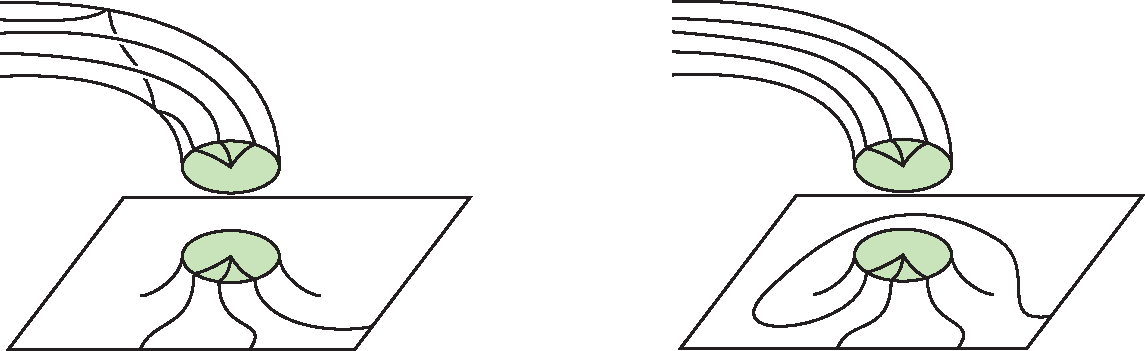
\includegraphics[scale=0.6]{OneHandlevsTetPivot.pdf} 
\caption{\label{OneHandlevsTetPivot}
\davex{Caption: ``A 1-handle and its attaching region on an adjacent 0-handle.
Standardizing the 0-handle attaching regions to be ``pitchforks" requires that we either have to add pivots to the 1-handle (left) or to the adjacent 0-handle (right). 
In \eqref{bos_tv_sum_std} we choose to include the pivots with 1-handles."}}
\end{centering} 
\end{figure} 

\medskip

These standardizations also serve to make the original state sum \eqref{bos_tv_sum} more uniform.
We can now write
\be \label{bos_tv_sum_std}
	Z(M) = \sum_{\beta\in\mcl(\mch)}
		\prod_{c\in\mch_3} \mcd^{-2}
		\prod_{f\in\mch_2} d(f, \beta)
		\prod_{e\in\mch_1} \Theta(P_e, \beta)^{-1}
		\prod_{v\in\mch_0} \text{Tet}(v, \beta) .
\ee
Here $\Theta(P_e, \beta)$ is a standard pairing as in \eqref{reflection_pairing_defn}, but modified by the pivot isomorphism $P_e$.
The weight $\text{Tet}(v, \beta)$ is a standard tetrahedral symbol (though there are still variants which depend on
the orientations of the edges of the tetrahedron).
The point is that we have now written the state sum for an arbitrary 3-manifold in terms of a finite number
of standard weights.



%%%%%%%%%%%%%%%%%%%%%
\subsection{The fermionic state sum}
%%%%%%%%%%%%%%%%%%%%%

\subsubsection{Definition of the fermionic state sum}

We now extend the bosonic state sum to the fermionic case. 
We start with two pieces of data: a super pivotal fusion category $\spc$, and a spin % spin implies oriented
3-manifold $M$ possessing a cell decomposition with orientations of 1- and 2-cells.
%The fermionic version of the state sum can be computed using similar techniques as in the bosonic case,
%and takes the form
The fermionic version of the state sum is similar to the bosonic version:
\begin{align}
\label{fermionic_tv_sum}
	Z(M) = \sum_{\beta\in\mcl(\mch)}(-1)^{\kappa_\beta}
		\prod_{c\in\mch_3} \mcd^{-2}
		\prod_{f\in\mch_2} \frac{d(f, \beta)}{n(f,\beta)}
		%\prod_{e\in\mch_1} \frac{ (-1)^{F(e,\sigma, \beta)}}{ \widetilde \Theta(e, \beta)}
		\prod_{e\in\mch_1}  \widetilde \Theta(e, \beta)^{-1}
		\prod_{v\in\mch_0} \text{Link}(v, \beta) .
\end{align}
There are several important -- often subtle --  differences built into the fermionic state sum which don't appear in the bosonic one, namely:
\begin{itemize} 
\item %The 0- and 1-handle weights are linear functionals on super vector spaces and as such have a sign ordering associated to each tensor.
The the string nets corresponding to the 0- and 1-handle weights require a sign-ordering of their string net vertices. 
This in turn requires that the partition function is weighted by a Koszul sign $(-1)^{\kappa_\beta}$
which measures the difference between the global sign ordering coming from the 1-handles and the global sign ordering coming from the 0-handles.
%\dave{That's a nice way to phrase it.}
\item The weights assigned to the 2-handles need to be properly normalized, 
resulting in a factor of $n(f,\beta) = \dim \End(a)$ if $a$ is the simple object labeling the core of the attaching annulus for the 2-handle $f$ by $\beta$.
%\item The spin structure on $M$ is determined by the spin structure on the 0- and 1-handles, 
%and correspondingly one needs to account for the possible application of the spin flip functor 
%when rigidly translating the vector space from the initial end of the 1-handle, 
%to the terminal end.
%\kw{Strictly speaking, this only applies after we have standardized}
\item The spin structure on $M$ determines how the basis elements which make up the labeling $\beta$ are inserted into
the graphs $\text{Link}(v)$.
\end{itemize} 
As in the previous section, we will now explain 
%and motivate 
the factors appearing in \eqref{fermionic_tv_sum}. 

%\begin{itemize} 
%\item The partition function is weighted by a Koszul sign and each local weight
%is computed with a Koszul ordering. In order to compute these Koszul signs, we need to assign an ordering to each of the vector spaces 
%appearing in the Hilbert space of the problem. 
%\dave{I think we should say something like `the partition function is weighted by a Koszul sign and each local weight is sign ordered.'}
%\ethan{Sounds good to me---changed the wording slightly}
%\dave{Need to say ordering on what.
%I would be inclined to say that we need an ordering for every tensor. 
%And then give a prescription to contract over tensors and find a possibly large tensor, with another ordering.}
%\item Since simple objects in $\spc$ can have non-trivial endomorphism algebras, some additional care must be taken to ensure the proper normalization of the partition function. 
%This is done by normalizing the 2-handle weights by a factors of $\langle \cl_B(x), \cl_B(x) \rangle$.
%\dave{Maybe we should say `...endomorphisms algebras, the 2-handle weights have to be normalized by $\langle \cl_B(x), \cl_B(x) \rangle$' or something similar.}
%\item Because of the relation $P^3 = (-1)^F$ in the fermionic case, care must be taken when implementing pivots during 
%standardization procedures. 
%\end{itemize}


\begin{comment}
things Dave wrote that essentially all appear in the section
\begin{itemize}
\item $n(f,\beta) = \dim \End(a)$ if $a$ is the simple object labeling the attaching region core of the attaching annulus for the 2-handle by $\beta$.
\item pairing on initial and terminal disks as determined by the 1-handle is sign ordered.
Lets choose the initial disk to have a lower sign ordering than terminal disk.
Note that this satisfies the spherical symmetry.
\item Each $\text{Link}(v)$ is also equipped with an ordering on the vertices.
A labeled$\text{Link}(v, \beta)$ is sign ordered according to the ordering of the vertices on $\text{Link}(v)$.
\item \dave{A possible way of determining the Koszul sign.}
The Koszul sign is determined as follows:
We choose an arbitrary global ordering the 0- and 1-handles. 
This determines a global ordering of the fermions on the attaching regions of the 0- and 1-handles. 
$\kappa_\beta = $  the number of Koszul isomorphisms needed in order to have the global ordering of the attachment regions in the 0- and 1-handles match.
\end{itemize} 
\end{comment}


%After accounting for these modifications, the state sum can be written as
%\begin{align}
%\label{fermionic_tv_sum}
%	Z(M) = \sum_{\beta\in\mcl(\mch)}(-1)^{\kappa_\beta}
%		\prod_{c\in\mch_3} \mcd^{-2}
%		\prod_{f\in\mch_2} \frac{d(f, \beta)}{n(f,\beta)}
%		\prod_{e\in\mch_1} \widetilde\Theta(e, \beta)^{-1}
%		\prod_{v\in\mch_0} \text{Link}(v, \beta) .
%\end{align}
%In the manner of the discussion in the previous section, we will now explain and motivate the factors appearing in the above formula. 

As before, we use the 2-cell orientations to define an oriented graph (unlabeled string net) on the boundary of each 0-, 1- and 2-handle.
String net graphs are assigned to the $k$-handles in the same way as in the bosonic case. 
The set of all labelings $\mcl(\mch)$ is defined as the product over all 1-handles $e$ of the basis sets $B(e)$.
For a fixed labeling $\beta \in \mcl(\mch)$, the weights are determined as follows.
%\kw{maybe say here that we choose sign-orderings?}
%\ethan{I was thinking that in this case, $\beta$ contains both a string-net labelling and a sign-ordering labelling}
%\dave{Do you mean sign orderings for each 0- and 1- handle? 
%We could do that. 
%I would like to avoid giving $\beta$ a sign ordering and keep it the way we have it, i.e., give a global ordering to the 1-handles and 0-handles.}
%\ethan{Right, I was essentially advocating for a notation where the choice of global ordering is contained in $\beta$}
%together
%with a choice of Koszul ordering for the ends of every 1-handle. 
%Note that since each 
%1-handle end is identified with a trivalent vertex on a 0-handle string net, such a Koszul 
%ordering also determines a Koszul ordering on the 0-handle string nets. 

The 2-handle weight $d(f, \beta)$ is defined in the same way as before. 
However we now divide by the factor $n(f, \beta) = n_a = \dim\End(a)$,
where $a$ the the simple object labeling the boundary of the core of the 2-handle.
This factor is necessary because the norm-square of the $a$-labeled loop is $n_a$.
%However, 
%%in order to ensure the proper normalization of the partition function, 
%%\dave{When I read normalization of partition function I think of overall normalization}
%we divide
%by the dimension 
%of the endomorphism algebra of the simple object that labels the core of the attaching annulus associated with the 2-handle $f$ by $\beta$. 
%This consideration is responsible for the factor of $n(f,\beta)$ appearing 
%in the 2-handle weight, 
%which is defined by $n(f,\beta)=\dim \End(a)$ for $f$ and $\beta$
%such that $d(f,\beta)=d_a$. 

%\kw{some rewriting starting here; D and E should review}
%\dave{I like it. I got a little confused in the Koszul sign discussion, I thought a simple picture would help (see below). 
%But I do like the way it's presented.}
%\ethan{made some small edits}

The 1-handle weights are determined by the bilinear pairings given by each 1-handle $e$. 
When evaluating the graph on the boundary of $e$, we choose the Koszul ordering which puts the terminal vertex
immediately before the initial vertex in the ordering (similar to the convention in \eqref{reflection_pairing_defn}).

For each 0-handle $v$, $\text{Link}(v,\beta)$ is defined in the same way as in the bosonic case:
we evaluate a string net determined by the 1- and 2-handles incident on $v$ and the labeling $\beta$.
There are two subtleties here.
First, when mapping a vertex label $\mu$ from the initial (terminal) end of a 1-handle to the opposing 0-handle adjacent to the terminal (initial) end of the 1-handle, 
we must employ the attaching map which connects the terminal (initial) end of the 1-handle to the 0-handle.
This attaching map is a spin diffeomorphism, 
and changing the attaching map by a spin flip changes the sign
of the label on the 0-handle by $(-1)^{|\mu|}$.
%%KW doesn't make sense to talk about $(-1)^F$ unless we already have another vertex label on the 0-handle that we are comparing to; but we don't have such
%the action of which is either trivial or the spin flip functor $(-1)^F$.
%If it is $(-1)^F$, the string net vertex label on the 0-handle needs an additional factor of $(-1)^{|\mu|}$.
It is here (and only here) that the state sum is sensitive to the spin structure on $M$.
%, which determines 
%the choice of $1$ or $(-1)^F$.
The second subtlety concerns Koszul orderings.
In order (pun noticed but not intended)
to evaluate the string net on the boundary of the 0-handle, we must choose an (arbitrary) ordering
of the string net vertices of the graph on the boundary of the 0-handle.
Thus the evaluation $\text{Link}(v, \beta)$ is arbitrary up to a sign.
However, we will see that a change of Koszul ordering which changes the sign of $\text{Link}(v, \beta)$ also produces a compensating
change in the factor $(-1)^{\kappa_\beta}$, and so the overall state sum is well defined.

\begin{figure} 
\centering
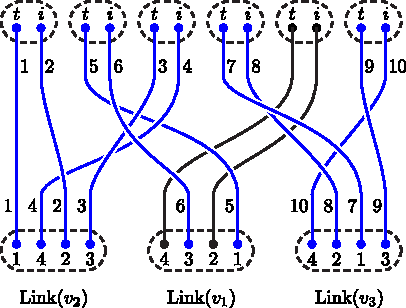
\includegraphics{KoszulFig.pdf} 
\caption{\label{KoszulFig} 
An example of how to compute the Koszul sign $(-1)^{\kappa_\beta}$ diagrammatically  
for a graph consisting of three 0-handles and six 1-handles. 
The lower dashed regions represent the 0-handles, while the upper dashed regions 
represent the 1-handles (with initial and terminal ends marked as $i$ and $t$, respectively). 
The Koszul orderings indicated by the numbers are explained in the text, and 
$\kappa_\beta$ is given by the number of crossings of the blue strands (in this example, 
$(-1)^{\kappa_\beta}=-1$).
\kw{I think we should add crossings between blue strands from different 0-handles, and draw in the even (non-blue) strands}
\davex{Sure.}
\kw{Also, I would indicate an ordering of all the strands, not just the odd ones.}
\davex{I think this messes things up a little. 
e.g., the even vertices on $\text{Link}(v_1)$ don't need to have adjacent ordering, but the 1-handle they are matched with does. 
So the black lines don't match up (unless I am doing something stupid)}
}
\end{figure}


The Koszul sign $(-1)^{\kappa_\beta}$ is defined as follows.
Consider, for fixed $\beta$, the tensor product of the all the super vector spaces
associated to the attaching disks on all the 0-handles.
If there are $k$ 1-handles, then there are $2k$ tensor factors in this tensor product, one 
for each 1-handle end. 
We will compare two different orderings of the tensor factors.
In the first ordering, we place each terminal disk immediately before each initial disk in the ordering.
Such an ordering is well-defined up to even permutations.
In the second ordering, 
we choose a global ordering of the 0-handles and then
use the above choices of local ordering for the factors associated to
each 0-handle
(this is again well-defined up to even permutations, since each 0-handle graph evaluates to zero when the total
parity at that 0-handle is odd).
We then define $(-1)^{\kappa_\beta}$ to be Koszul sign relating these two orderings. 

\medskip

\kw{Note to self: review below again after edits}

We now describe a convenient way to compute $(-1)^{\kappa_\beta}$ graphically, with an 
example shown in Figure \ref{KoszulFig} for a graph consisting of six 1-handles (upper dashed regions) and 3 0-handles $v_1,v_2,v_3$ (lower dashed regions). 
Each 0-handle has four 1-handle attaching regions, which are indicated by the lower small dots and 
which possess an ordering relative to one another (indicated by the numbers within the lower dashed regions). Each attaching 
region can either be even (black) or odd (blue). If it is odd, 
\kw{I would assign, regardless of oddness}
we assign a Koszul ordering to the attaching
region, indicated by the numbers appearing just outside the lower dashed regions.

Each 1-handle either has two even ends or two odd ends: if it has two odd ends, we assign an ordering 
to the ends by placing the terminal end immediately before the initial end in the ordering. This ordering
is denoted by the top row of numbers below the 1-handles in Figure \ref{KoszulFig}. 

To evaluate $(-1)^{\kappa_\beta}$, we draw a fermion line connecting each odd 0-handle attaching region
with Koszul order $k$ to the respective 1-handle end with Koszul order $k$. $(-1)^{\kappa_\beta}$ is then 
simply $(-1)^{n_c}$, where $n_c$ is the number of crossing between fermion lines in the resulting diagram. 
In the example of Figure \ref{KoszulFig} we have $n_c=11$, and so $(-1)^{\kappa_\beta}=-1$. 

\medskip

The case of non-empty $\bd M$ presents one new issue not present in the bosonic version:
we must pick a Koszul ordering of the labels corresponding to string net vertices on $\bd M$.
Once this has been done, we can combine that ordering with the ordering coming from the 1-handles.
The Koszul sign $(-1)^{\kappa_\beta}$ is now defined to be the sign arising from comparing 
the 0-handle ordering with the combined $\bd M$ and 1-handles ordering.

%\kw{we should probably say something about the case with boundary.
%at least discuss the Koszul ordering issues.}
%\dave{I agree, can attack this once re-visiting the bosonic case.}
%\ethan{discussion about boundaries and wavefunctions already kinda exists at the end of the fermionic tensor network part}






\begin{comment}	%% Dave's older version  %%%%%%%%%%%%%%
\dave{Admittedly, this does standardize the 1-handles.
I think it's less confusing when we write down the tensor network to explicitly have the parity matrices on the edges.}
The 1-handle weights are determined by the bilinear pairings given by each 1-handle $e$. 
This pairing is defined by rigidly translating the intitial disk through the 1-handle and and gluing it to the terminal disk across a 2-sphere (with the initial disk having a lower Koszul ordering than the terminal disk).
%This pairing is found from gluing the initial disk to the terminal disk on a sphere and evaluating the net after a translation through the 1-handle. 
While gluing across the 2-sphere it is possible that the spin structures of the two disks differ by a spin automorphism (whose action is encoded in the spin flip functor $(-1)^F$).
\dave{We could also take a path that parallels the edge term in the Hamiltonian section.
} 
%The net to be evaluated is defined with a lower koszul ordering on the initial disk than the terminal disk. 
This spin automorphism is defined by the 1-handle $e$ and the spin structure $\sigma$.
We explicitly write the action of the spin automorphism as $(-1)^{F(e, \sigma)}$ so that the 1-handle weights take the form $(-1)^{F(e,\sigma, \beta)}/\widetilde{\Theta}(e, \beta)$. 
Where $\beta$ is the the labeling of the initial disk, and $F(e, \sigma, \beta)$ is $0$ if $\beta$ has even fermion parity, and $1$ if $\beta$ is odd, 
and the spin structure on the initial and terminal disk differ by a spin flip functor.

%As in the bosonic case, $\widetilde\Theta(e, \beta)$ is defined by the value of the bilinear pairing evaluated on $\mu^*$ and $\mu$, where $\mu^*$ $(\mu)$ 
%is a basis vector in the Hilbert space of the initial (final) attaching end of the 1-handle 
%$e$. In the fermionic case, each vector comes with a Koszul ordering, and 
%we define $\widetilde\Theta$ to only act on edges such that the Koszul ordering
%of the vector $\mu^*$ labeling the initial end of $e$ is exactly one less than that of the vector $\mu$
%labeling the terminal end of $e$. 
%For example, if $e$ has four adjacent 2-handles labeled by $a,b,c,d$ with the orientations of Figure \ref{OneHandlePrime} so that $\mu \in V^{ab^*c^*d}$, then we have \ethan{Dave, would you mind adding a koszul ordering of $k$ to $\mu^*$ (the initial disk vector) and an ordering of $k+1$ to $\mu$ (the terminal disk vector)?}
%\be \widetilde \Theta (e, \beta) =  \Bananafourmu,
%\ee
%where the Koszul ordering is indicated explicitly by the numbers located next to the vertices. 

Additionally, for each 0-handle $v$, $\text{Link}(v,\beta)$ is defined in the same way as in the bosonic case (namely, as the evaluation of a net determined by the 1-handles incident on $v$), 
although now for the evaluation of $\text{Link}(v,\beta)$ to be defined we need to assign an ordering to the vertices of the graph $\text{Link}(v)$.
The 0-handle weights are the evaluation of $\text{Link}(v, \beta)$ with the sign ordering determined by the ordering of the vertices of $\text{Link}(v)$.

Lastly, 
we need to define the Koszul sign $(-1)^{\kappa_\beta}$, whose sole job is to compensate for the arbitrary sign ordering we've given each of the vertices on the 0-handle graphs $\text{Link}(v)$. 
To do so, we first give a global ordering to the 0- and 1-handles.
This then determines a global ordering of the fermions on the 0-handles (since each 0-handle is ordered), 
and independently a global ordering of the fermions on the 1-handles (since each 1-handle is sign ordered from initial to terminal).
We then have,
\begin{align}
(-1)^{\kappa_\beta} = \text{sign} (\sigma)
\end{align}
Where $\sigma$ is the permutation needed to have the two global orderings match (equivalently, $\text{sign}(\sigma)$ is the number of transpositions needed for the two sign orderings to match modulo two). 
Additionally, two global orderings of the 0-handles (1-handles) are related by an even number of transpositions in the sign ordering, 
and so the sign $(-1)^{\kappa_\beta}$ is independent of both global orderings.
Furthurmore, the partition function is independent of the arbitrary ordering assigned the vertices of the 0-handle graphs $\text{Link}(v)$.
To see this, we note that if we change the ordering of the vertices of $\text{Link}(v)$ by a single transposition, then the weight itself will pick up a negative sign (if both labels are odd), 
and the we will have to do one extra transposition to determine the Koszul sign $(-1)^{\kappa_\beta}$. 
Hence the two signs cancel.
(if both or one of the labels are even then the transposition of the ordering in that given 0-handle has no effect on the Koszul sign or the 0-handle weight).
\end{comment}	%% end Dave's older version  %%%%%%%%%



\begin{comment} %%%%%%%%%%%%%%%%
\dave{Plan is to move the following to scrap notes.}
\dave{I am skeptical of the following, 
but wanted to write down the idea while I was thinking about it.
}
We also note that $(-1)^{\kappa_\beta}$ can be written as the evaluation of a diagram in $\text{sVec}$.\footnote{The braided fusion category $\text{sVec}$ has two simple objects which we denote $\unit$ and $\psi$. 
$\psi$ has $\zt$ fusion rules, trivial F-symbols and is a fermion.}
This has the advantage of implicitly modding out by even permutations, and does not require a global ordering of the 0- and 1-handles. 
For each 1-handle that has an odd parity initial disk we draw a graph on the plane with two vertices and one edge labeled by $\psi$.
Next we draw the graphs $\text{Link}(v)$ on the plane. 
We now connect pairs of vertices on $\text{Link}(v)$ with $\psi$ lines if they have odd parity (it is important that no braids are introduced). 
We now ``connect'' the two planar graphs with $\psi$ lines, and evaluate the diagram, see Figure \ref{sVecFig} for an example.
(Note that we are actually taking an inner product between the planar graph defined by the 1-handles, and the planar graph defined by the 0-handles)
\end{comment} %%%%%%%%%%%%%%%%


%%old svec fig
\begin{comment}
\begin{figure}
\begin{centering}
\begin{align}
\nonumber
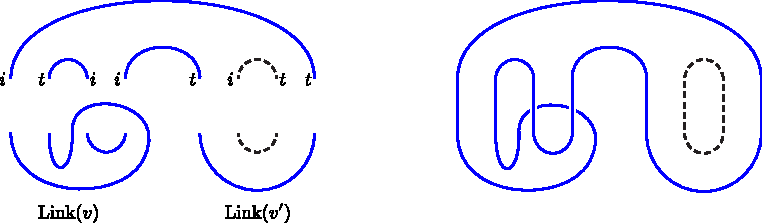
\includegraphics{sVecFig.pdf}
\end{align}
\end{centering} 
\caption{\label{sVecFig}
An example of a Koszul sign $(-1)^{\kappa_\beta}$ written as the evaluation of a diagram in $\text{sVec}$ for a pair of two vertices $v,v'$. 
The upper half of the left figure denotes the 1-handles, with $i$ ($t$) marking the initial (terminal)
edge of the 1-handle.  
The lower half of the left figure shows the two 0-handles, which each have four attached 1-handles.
Solid lines are labeled by $\psi$ and connect two fermion dots with adjacent sign ordering, while dashed lines denote the trivial object. 
The right figure shows the diagram in sVec obtained after connecting the strings on the 0-handles to 
the respective strings on the 1-handles; the evaluation of this diagram determines $(-1)^{\kappa_\beta}$. \ethan{changed the caption a bit to hopefully be a bit clearer}
}
\end{figure}
The evaluation of the diagram can be written as a TVBW state sum, but since we have written the evaluation on the plane, it doesn't sit naturally with the TVBW state sum \eqref{fermionic_tv_sum}.
\dave{Intuition, but haven't checked (Maybe this is Kapustins shadow thing; see \cite{bhardwaj2016}?): 
The combination $(-1)^{\kappa_\beta}(-1)^{F(e, \sigma,\beta)}$ can be written as a TVBW state sum on $M$ with $\mcc = \text{sVec}$.
}
\dave{Could think about:
If $\spc$ is dervied through a fermionic quotient then the parition function can be written as$\cdots$. 
If the Manifold has Boundary then $\cdots$}
\end{comment}


%For a given labeling $\beta\in\mcl(\mch)$, the Koszul ordering assigned by $\beta$ will not generically be 
%compatible with the condition needed to evaluate $\widetilde\Theta$. 
%We define the 1-handle Koszul sign $(-1)^{\kappa_1}$ to be the sign picked up when 
%permuting the given Koszul order into one for which the $\widetilde\Theta$ can be evaluated.
%That is, $(-1)^{\kappa_1}$ is equal to $(-1)^{{\rm sgn}(\sigma)}$, where $\sigma$ is the 
%permutation sending the input Koszul ordering determined by $\beta$ to one in which 
%for every 1-handle whose initial disk has Koszul order $k$, the terminal 1-handle has Koszul 
%order $k+1$. 

%Finally, for each 0-handle $v$, $\text{Link}(v,\beta)$ is defined in the same way as in the bosonic case (namely, as the evaluation of a net determined by the 1-handles incident on $v$), although 
%now each vertex in the graph carries a Koszul ordering.  
%For a given choice of $\beta$, the Koszul ordering we are given will not generically 
%be one in which the 0-handle nets can be evaluated, since removing a pair of fermions 
%can only be done if the two fermions possess adjacent Koszul ordering (for example, we would not be able to evaluate a net containing two fermions with Koszul orders $k$ and $k+2$).
%We define the 0-handle Koszul sign $(-1)^{\kappa_0}$ to be equal to the Koszul 
%sign picked up when permuting the input Koszul ordering to one in which the string 
%nets at each 0-handle can be evaluated\footnote{Of course, there are multiple choices of Koszul orderings for which the 0-handle graphs can be evaluated, but 
%differences in the sign of $(-1)^{\kappa_0}$ between these orderings are compensated for 
%by differences in the signs of the ${\rm Link}(v,\beta)$ factors, so that the partition function 
%is insensitive to such choices.}.
%The total Koszul sign appearing in the partition function $Z(M)$ is then obtained 
%as $(-1)^{\kappa_\beta} = (-1)^{\kappa_0+\kappa_1}$.



%%%%%%%%%%%%%%%%%%
\subsubsection{The fermionic state sum as a tensor network}
%%%%%%%%%%%%%%%%%%

We now turn to the task of reinterpreting \eqref{fermionic_tv_sum} as a tensor network. %\ethan{replaced ``regularization'' with ``standardization'' since regularization has a different physics meaning}
%\dave{Definitely a good idea.}

\medskip

We incorporate the factors of $d(f, \beta)/n(f,\beta)$ and $\mcd^{-2}$ into the 0-handle 
weights 
in the same way as in the bosonic case. 
As in the bosonic case we denote the dressed 0-handle weights by $\widetilde{\rm Link}(v,\beta)$.
%Denoting the modified 0-handle weights by $\widetilde{\rm Link}(v,\beta)$, 
We define the vertex tensor in a similar fashion to \eqref{vertex_tensor}. 
Let $e_1, \cdots, e_k$ be the 1-handles adjacent to the 0-handle $v$ with the same ordering as the vertices of the graph $\text{Link}(v)$.
Let $V_i$ be defined in the same way as \eqref{0_handleVectorspaces} (with the modification that $V_i$ is a super vector space).
We define 
\begin{align} 
T_v  \in V_1^* \tp \cdots \tp V_k^*
\end{align}
by 
\begin{align}
T_v(w_1 \tp \cdots w_k) = \widetilde{\text{Link}}(v, w_1 \tp \cdots \tp w_k)
\end{align} 
where $w_i \in V_i$.
In words, $T_v$ evaluates the string-net graph determined by $\text{Link}(v)$ with the ordered vertices labeled by $w_1, \cdots, w_k$ (in the same order), and multiplied by the appropriate factors of $d(f,\beta)/n(f,\beta)$ and $\mcd^{-2}$.
%where the sum runs over a complete orthogonal basis of the attaching regions associated associated with the 0-handle $v$.
%where the sum runs over orthogonal basis vectors for the vertex Hilbert space $\mch(v)$. 
%For a 0-handle on which $n$ 1-handles terminate, the vectors $w_v$ admit a 
%decomposition $w_v = \bigotimes_{i=1}^n w_{v,i}$. 
%These vectors are assigned the same Koszul ordering as the ordering of the vertices on the $\text{Link}(v)$ graphs.
%These vectors are assigned Koszul ordering in the standard implicit left-to-right way. 
%\dave{Is this necessary?}
%\ethan{It was intended to be my guess to what Kevin's dual spaces comment meant. Might have missed the mark though, and it might still be confusing.}

%\kw{I've using ``Koszul ordering" rather than ``sign ordering" most of the time.
%A sign ordering is an ordering modulo even permutations, so it doesn't really make sense to say that two things are adjacent
%in a sign ordering.}
%\ethan{agreed}
%\davex{Sounds good. Thanks.}

%To obtain the partition function, we again form the tensor product of all the 0-cell tensors and contract over all indices.
As in the bosonic case, the partition function 
is computed as a trace of the $T_v$ tensors:
\be \label{fermion_Z_as_tr} Z(M) = \tr \left(\bigotimes_{v\in \mch_0} T_v\right).\ee
where the $\tr$ denotes contracting dual indices.
%where the trace is denotes denotes the sum over all contracted 1-cell labelings normalized by $\widetilde{\Theta}^{-1}$.
%The tensor trace is defined so that we insert a parity matrix $(-1)^{F(e, \sigma)}$ on every 1-cell, and a $\widetilde{\Theta}$ symbol normalization in the contraction. 
In practice, to perform the trace, we require that the pair of vectors to be contracted be adjacent in the Koszul ordering (with terminal preceding initial). 
%In practice, to perform the contraction, the we require the pair of vectors being contracted over to have adjacent Koszul ordering (i.e., initial to terminal).
To make the pair of vectors adjacent in the Koszul ordering we need to apply a number of Koszul isomorphisms. 
After contracting all vectors we pick up the appropriate factor of $(-1)^{\kappa_\beta}$. 
Again, $Z(M)$
is independent of the way we assign factors of $d(f,\beta)/n(f,\beta)$ and $\mcd^{-2}$ to the 
vertex tensors. 

If $\bd M$ is non-empty, we again follow the bosonic prescription in \eqref{trace_pM_nonempty} 
to obtain $Z(M) = \tr \left( \bigotimes_{v\in \mch_0} T_v \right) \in W_1^*\tp\cdots\tp W_n^*$, where 
$W_1, \ldots, W_n$ are the vector spaces associated to the boundary 0-cells and we 
are implicitly making use of the undordered tensor product. When using $Z(M)$ to compute 
amplitudes of different string-net boundary conditions, care must be taken when performing the 
tensor contraction on ordered representatives because of Koszul sign issues. 

\medskip

\kw{Let's discuss following on skype}

\ethan{un-commented the following since I still think we should include a contraction example, either here 
or possibly in defn section}

%In the above equation, the Koszul ordering of each tensor factor is determined in the usual implicit way, 
%so that it increases from left to right on the page (the ordering of the $T_v$ 
%tensors is determined by an arbitrary global ordering on the 0-cells). However, this left-to-right ordering will almost always not be 
%the ordering required in order to perform the tensor contraction (namely one where 
%vectors and their associated dual vectors are adjacent to one another in the tensor product). 
%Re-arranging the Koszul ordering given by the left-to-right convention produces a Koszul sign not
%present in the bosonic partition function (which appears as $(-1)^{\kappa_\beta}$ in \eqref{fermionic_tv_sum}).

We will now elaborate on how to perform tensor contractions in the fermionic setting. 
When we contract
%%KW I think "trace out" is idiomatic, but I've never heard "contract out".  I do hear plain "contract" (without the "out")
two tensor indices of a tensor in $\mch^*\tp\mch$, we must be careful to only perform 
the contraction on two tensor factors that have adjacent Koszul ordering in the tensor product.
For example, suppose we have two tensors $Q \in V_Q$ and $T\in V_T$,
defined by
\begin{align}
Q &= \sum_{q_L \tp q \tp q_r } Q(q_L \tp q \tp q_R)q_L \tp q \tp q_R,\\
T &= \sum_{t_L \tp t \tp t_R} T(t_L \tp t \tp t_R  )t_L \tp t \tp t_R,
\end{align}
where we have split the vector spaces $V_Q$ and $V_T$ into tensor factors on 
the left and right of the two indices that we would like to contract, namely $t \in V$ and $q \in V^*$.
We define the contracted tensor by $K$, which is given by
\begin{align}
K = \sum_{ q_L \tp q_R \tp t_L \tp t_R}K(q_L \tp q_R \tp t_L \tp t_R) q_L \tp q_R \tp t_L \tp t_R,
\end{align} 
with 
\begin{align}
\label{contraction_example}
K(q_L \tp q_R \tp t_L \tp t_R) &= \sum_{q,t} Q(q_L \tp q \tp q_R)R(t_L \tp t \tp t_R  ) (-1)^{|q| |q_r|}(-1)^{|t_L| | t|} \delta_{q^*,t}\\
&= \sum_{t} Q(q_L \tp t^* \tp q_R)R(t_L \tp t \tp t_R  ) (-1)^{|t|( |q_R| +|t_L|)}.
\end{align}
In the above, we have used the fact that $\delta_{q^*,t}$ is only non-zero
if $|q|=|t|$. 
The Koszul sign $(-1)^{|t|( |q_R| +|t_L|)}$ is picked up from commuting the tensor factors $q$ and $t$ next to one another, so that they have the correct Koszul ordering for being input into the contraction map. 

\ethan{I found the following very useful for avoiding confusion, but it's likely not strictly needed}
In the above examples, we have used the implicit left-to-right Koszul ordering convention.
In practice, we will more often be performing a contraction on a series of tensors whose Koszul
orderings are indicated explicitly by numerical subscripts, since this notation is better suited to 
our diagrammatic formalism. For example, we have 
\be Q\tp T = \sum_{q_L \tp q \tp q_r } Q(q_L \tp q \tp q_R)T(t_L \tp t \tp t_R  ) q_{L1} \tp q_2 \tp q_{R3} \tp t_{L4} \tp t_5 \tp t_{R6}.\ee
We would like to contract out the indices $t\in V,q\in V^*$, but in order to do this they must have adjacent Koszul ordering. 
To obtain such an 
order, we use the following manipulations:
\begin{align} q_2 \tp q_{R3} \tp t_{L4} \tp t_5 & = (-1)^{|q||q_R|}q_3 \tp q_{R2} \tp t_{L4} \tp t_5 \\ & = (-1)^{|q||q_R|+|t||t_L|} q_3 \tp q_{R2} \tp t_{L5} \tp t_4.
\end{align}
We are now ready to contract out the $q$ and $t$ indicies. The Koszul sign we pick up, namely 
$(-1)^{|q||q_R|+|t||t_L|}$, is of course the same as the one obtained with the implicit left-to-right Koszul ordering convention. 

In summary, the Koszul sign that appears when performing the tensor contraction in the evaluation of $Z(M)$ can be found 
by ensuring that tensor factors 
being contracted always have adjacent Koszul-ordering and by using \eqref{contraction_example} repeatedly.



%%%%%%%%%%%%%%%%%%%%
\subsubsection{Fermionic standardization procedures}
%%%%%%%%%%%%%%%%%%%%

\kw{some new material here}
\davex{Looks good to me, added `we' to the first sntence.}
As in the bosonic case, we can standardize the tensor network by
choosing a generic cell decomposition (dual to a triangulation)
and ``pitchforkizing" all trivalent vertices which appear on the boundaries of 0-handles.
Note that in this fermionic setting, pitchforkizing includes choosing a spin framing at each trivalent vertex.
%As in the bosonic case, we may employ a standardization 
%procedure in which 
%the cell decomposition is generic (dual to a triangulation) and
%all vertices in the string nets assigned to the 0-handles are in the pitchfork form.
This standardization procedure results in string net vertices on 0-handles which are standardized independently of their partners at the opposite
ends of the 1-handles: 
the form of a given trivalent vertex at the initial edge of a 1-handle $e$
and the form of the associated vertex on the terminal edge of the 1-handle may be related by a pivot operation.
Properly accounting for this requires inserting pivot operators $P_e=P^{l_e}$ into the 
1-handles, as in \eqref{horshoe_resln}. 
Rather than tacking the spin-structure signs onto the 0-handle weights 
%(as we did in the state sum described above) 
we incorporate them into the pivots.
Indeed, we now have $P_e^3=(-1)^F$, so that $l_e$ is 
valued in $\zz_6$ as opposed to $\zz_3$ (alternatively, we could keep $l_e \in \zz_3$  but insert $(-1)^{F} \cdot P^{l_e}$ where appropriate).
%We keep the spin framing at the 0-handles fixed by virtue of the pitchforkization procedure (and require that every 0-handle is related by a translation), 

Note that the spin structure of the underlying 3-manifold is encoded in the edge pivots $P_e$ (and the standardized 0-handles).

%\dave{The following may need to be done more carefully}
%The attachment regions of the 0-handles are also related by spin diffeomorphisms, 
%in this case either $\text{id}$ or $(-1)^F$. 
%If we multiply all the pivots along a closed path (including those coming from the 0-handles) then they must equal $(-1)^F$ if the 
%path is bounding and $+1$ if the path is non-bounding.
%\dave{Is it that simple?
%I thought we would have to say something about transporting the fermions through the 0-handles 
%(e.g., a sloppy argument is to introduce a trivial branch sheet \ethan{??} on every 0-handle and slide it over one of the attaching disks. 
%This means each 1-handle picks up an extra factor of $(-1)^F$, and so if there are an odd number of 1-handles on the path they don't all cancel).} 
%\dave{I thought branch sheet was the appropriate word to use for 3d.}


%Lastly, we note that if we further require the cell decomposition to be dual to a triangulation, 
%then we can choose the 0-cell weights to that a take a form similar to \eqref{Bosonic_tet}.
%The modification is that the vertices of $\text{Link}(v)$ must be ordered, 
%so that 
The standard tetrahedral string net on each 0-handle must of course incorporate a Koszul ordering in the fermionic case: 
\begin{align} 
	%T_v = \TetrahedronPrime \; \cdot \alpha \tp \beta \tp \gamma \tp \delta, 
	T_v(\alpha \tp \beta \tp \gamma \tp \delta) = {\rm Tet}(v,\alpha \tp \beta \tp \gamma \tp \delta) = \Tetrahedron.
\end{align}
Note that there are still multiple versions of the standardized tetrahedral weights ${\rm Tet}$ differing by choices of the edge orientations.
The fermionic analogue of \eqref{bos_tv_sum_std} can now be written:
\begin{align}
\label{ferm_tv_sum_std}
	Z(M) = \sum_{\beta\in\mcl(\mch)}(-1)^{\kappa_\beta}
		\prod_{c\in\mch_3} \mcd^{-2}
		\prod_{f\in\mch_2} \frac{d(f, \beta)}{n(f,\beta)}
		%\prod_{e\in\mch_1} \frac{ (-1)^{F(e,\sigma, \beta)}}{ \widetilde \Theta(e, \beta)}
		\prod_{e\in\mch_1}  \Theta(P_e, \beta)^{-1}
		\prod_{v\in\mch_0} \text{Tet}(v, \beta) .
\end{align}
Again, $\Theta(P_e, \beta)$ is a standard pairing as in \eqref{reflection_pairing_defn} but modified by the pivot isomorphism $P_e = P^{l_e}$.

\begin{comment}
OLD STUFF BELOW:
\kwsep 

%%%%%%%%%%%%%%%%%%%%%%%%%%%%%%
\subsection{Notation, standardization, and Hilbert spaces}
%%%%%%%%%%%%%%%%%%%%%%%%%%%%%%

\kw{Do we need to make it clearer that we are reviewing the bosonic case as a warm-up here?
I was confused on this point.}

In this section we will review the construction of the bosonic state-sum as a warm up, and we 
will do it in a way that readily generalizes to the fermionic setting. 

We start with two pieces of data: 
\begin{itemize}
\item a spherical fusion category $\mcc$, 
\item and an oriented 3-manifold $M$ 
%\kw{I think we should consider changing the to $M$.  We usually use the mathcal letters for categories and plan letters for manifolds.}
%\ethan{agreed, changed.}
possessing a cell decomposition with oriented 2-cells 
%\kw{We should think about whether a plain (non-transverse) orientation would be more convenient}
and oriented 1-cells. 
\end{itemize}
In what follows, we will assume that $M$ is closed for simplicity. We will drop this 
assumption when we discuss wave functions and the shadow world construction. 

Our first order of business is to fatten the cell decomposition into a handle decomposition, 
as was done in Section \ref{standardized_handles}.
\dave{Moved the following bit to handle decomposition section.}
Recall that a handle decomposition for a 
3-manifold $M$ is built from a series of $k$-handles, with $k=0,1,2,3$, each of which is identified with $D^k\times D^{3-k}$). 
We will often refer to a $k$-cell and its associated $k$-handle with the same letter. 
We call $S^{k-1} \times D^{3-k}$ the attaching region (or attaching boundary) of the $k$-handle,
and $D^k\times S^{3-k-1}$ the non-attaching boundary.
%The attaching region of a $k$-handle is $S^{k-1} \times D^{3-k}$,
The attaching map of a $k$-handle is a homeomorphism from the attaching region to 
a submanifold of the boundary of the union of the lower-dimensional handles.
The topology of $M$ is encoded by the various attaching maps.
%is built into the attaching regions where different handles are connected, each of which is homeomorphic to $S^k \times D^{n-k}$.
%We are interested in 3-manifolds,
%and hence the attaching regions between between the $(k+1)-$ and $k$-handles are given by
%$S^2 \times D^0$ (3-handles to 2-handles), $S^1 \times D^1$ (2-handles to 1-handles), and $S^{0} \times D^2$ (1-handles to 0-handles).
%%KW k-handles attach to the boundary of the 0, 1, ... k-1 handles, not just the k-1-handles
Although not necessary, we assume the cell decomposition of $M$ is dual to a triangulation for ease of notation.
The standardization procedure is similar to the pitchforkization procedure defined in \eqref{pitchfork_basis} and surrounding text.

%To define the tensors in \eqref{TVBWss} explicitly, 
%it is helpful to standardize each of the cells, 
%and the vector spaces we assign to each cell. 
%Technically, the partition function is built on a handle decomposition, 
%but its useful to label the data associated to each handle by the corresponding cell. 



%\ethan{tried (valiantly) to make this more comprehensible, but may have not fully succeeded} 
%\dave{A valiant effort indeed.}


We first establish some notation for the attaching regions of the $k$-handles, which are summarized 
in Figure~\ref{NotationStateSum}. 
We denote the collection of 2-cells by $\mcf$, the collection of 1-cells by $\mce$, and the collection of 0-cells by $\mcv$.
Each $f \in \mcf$ is homeomorphic to a polygon, see `f' in Figure~\ref{NotationStateSum}.
The orientation of $f$ induces an orientation of each edge of the polygon .
%(equivalently, we could say each 2-cell is equipped with a boundary orientation, rather than a transversal orientation).
%Each edge of $f$ is oriented by the orientation assigned to $f$.% (equivalently, each 2-cell is equipped with a boundary orientation).
%We will denote the edge $e$ at the boundary of the 2-cell $f$ by $c_{fe}$.
We will denote the edge at the boundary of the 2-cell labeled $f$ by $c_{fe}$, 
where $e$ is the 1-cell which it attaches to.
(Note the the orientation of the 2-cell and orientation of the 1-cell are chosen independently.)


The 1-handle associated to an edge $e$ intersects three adjacent 2-handles.
%The tubular neighborhood of a given 1-cell $e$ is a 1-handle which intersects three neighboring 2-cells.
% in a collection of three rectangles. %On any given $D^2$ cross-section of 
%a 1-handle, these intersection regions meet at a trivalent vertex. %connected by an annulus with three oriented lines.
The non-attaching boundary of each 1-handle comes equipped with three oriented lines, which match up with 
the edges of the three 2-cells whose boundaries include the 1-cell $e$. For an 
illustration of this, see Figure \ref{One_handle}. 
%The intersections of the three 2-cells with the surface of the 1-handle consists of three lines, 
The orientation of these lines is defined to be opposite to that of the neighboring 2-cell boundaries.
We denote the edge on the boundary of a 1-handle $e$ that matches up with a boundary component 
of the 2-cell $f$ by $\bar{c}_{fe}$, where the bar signifies that the orientation is opposite that of the edge of the 2-cell (see Figure~\ref{NotationStateSum}). 

A 1-cell $e$ connects two 0-cells, $v$ and $v'$. 
A $D^2$ cross-section of the intersection between a 1-handle $e$ and its three neighboring 2-cells 
is a disk with a trivalent vertex in its interior and three marked points on its boundary. 
We will denote the trivalent vertices appearing at either end of $e$ by $c_{ev}$ and $c_{ev'}$.
The orientations of the edges emanating from these vertices are determined by the neighboring 2-cells.
Again, see Figure~\ref{NotationStateSum} for clarification.

A small $S^2$ drawn around a 0-cell intersects six 2-cells and four 1-cells.
For our purposes, it is enough to keep track of the four neighboring 1-cells, 
since they contain all the orientation information that the 2-cells assign to the $S^2$ surrounding the 0-cell.
%Removing a single point from this spherical neighbourhood allows us to define a homeomorphism into the plane. 
%Furthurmore, the gluing regions for the 1-cells can all be taken to be pitchforks as in \eqref{pitchfork_basis}, see Figure~\ref{FIGURE}.
%This is our standardized 0-cell (actually spherical neighbourhood of the 0-cell). 
Denote the 0-cell by $v$ and the neighboring 1-cells by $e_j$, $j=1, \cdots 4$.
Each of the four 1-cells intersects the small $S^2$ at a point where three of the intersections of 
the six 2-cells with the $S^2$ meet. 
We denote these four trivalent junctions by $\bar{c}_{e_j v}$, 
and again the bar denotes that these are in the opposite orientation relative to the trivalent vertices $c_{e_jv}$ at the boundaries of the 1-cells. 

The Figure \ref{NotationStateSum} only shows one representative sample of cells, which all others are homeomorphic to. 
We now standardize each cell so that we can keep track of the topological data associated to the handle decomposition relative to a `standard' one. 
This is analogous to the pitchforkization procedure discussed in the text surrounding \eqref{pitchfork_basis}.
We first note that the spherical neighborhood of an arbitrary 0-cell $v$ can be standardized by removing a point and mapping the resulting picture to the plane. 
We can next `pitchforkize' the attaching region where the four 1-handles are attached to $v$ so that each take the form
\begin{align}
\StandardZeroCell,
\end{align}
or some variant thereof obtained by reversing the orientations of the edges. 
The dashed circles in the above equation are the attaching regions for the 1-handles and again, 
the lines in the above diagram represent the intersections of the six 2-cells 
with the spherical neighbourhood of $v$. 
%whose boundaries include $v$
%with the $S^2$ surrounding $v$. 
The numbers indicate which edge is connected to where on the standard 0-handle, and are associated with $\bar{c}_{e_j v}$.
\kw{I don't understand this last sentence.  What numbers?}

With this standardization procedure, 
the 1-handles which attach two 0-handles are now horseshoe-shaped.
Each 1-handle $e$ can be deformed into the following form:
\begin{align} \label{horshoe_resln} 
\HorshoeIdentity,
\end{align}
where $P_e$ is either the identity, $P$, or $P^2$, where $P$ is the pivot defined in \eqref{Pitchfork_pivot}.
We define $P$ to rotate diagrams counterclockwise relative to the orientation of $e$.
The possible presence of $P$ and $P^2$ is needed to keep track of any relative pivoting
between the pitchforks at either ends of the 1-handles. 


%end of notation bullshit 

%\dave{This sentence has a lot of enthusiasm.} \ethan{:)}
With our vast notational arsenal now fully developed and eager to be utilized, 
we are ready to assign vector spaces to each of the attaching regions $c_{xy}$ defined above.
We define the vector spaces 
\begin{align} \label{EandWdefns}
E = \bigoplus_{x\in\mcc} \cc_x \quad \quad \quad W = \bigoplus_{a,b,c\in\mcc}V^{abc}
\end{align}
where the sums are over a representative set of the simple objects in the input category $\mcc$. 
Momentarily, the vector space $W$ will be assigned to pitchforks.
Not all pitchforks will be oriented with all edges pointing outwards; in this scenario 
we repeat the construction in \eqref{pitchfork_basis} and replace an object labelling an inward-pointing 
edge with its dual. 
The vector space we assign to each of the attachment regions are as follows:
\begin{align}
\label{attaching_region}
  \mch(c_{fe}) &= E \quad \quad \mch(\bar{c}_{fe}) = \mch(c_{fe})^* = E^*\\
\mch(c_{ev} )&= \begin{cases} W &\text{if $e$ is oriented away from $v$} \\
W^* &\text{otherwise} 
\end{cases}\\
\mch(\bar{c}_{ev}) &= \mch(c_{ev})^*
\end{align}
\kw{Shouldn't we have 8 different versions of $W$?}
\dave{There are $8$ versions of it, which we left implicit (see sentences following \eqref{EandWdefns}).
The two referred to in this equation correspond to whether we take our standard basis (if the 1-cell is oriented away from $v$) our the dual basis (the 1-cell is oriented toward $v$).}
The vector space assigned to each $k$-handle is given by tensoring over the vector spaces assigned to each attachment region.
\kw{should say this a little differently; we said above that each k-cell has only one attaching region}
For a 2-handle $f$, a 1-handle $e$, and a 0-handle $v$, we have 
\begin{align}
& \mch(f) = \bigotimes_{c_{ef} \in \partial f} \mch(c_{ef}),  \\
& \mch(e) = \left(\bigotimes_{\bar{c}_{ef} \in \partial e }\mch (\bar{c}_{ef}) \right)\tp \mch(c_{ev}) \tp \mch (c_{ev'}), \\
& \mch(v) = \bigtp_{i=1}^4 \mch(\bar{c}_{e_{i}v}), 
\label{tensor_space}
\end{align}
where as before, $c_{ef} \in \partial f$ are the oriented attachment regions of the 2-cell labeled by $f$, 
and the $\bar{c}_{ef} \in \partial e$ are the lines on the surface of the 1-handle $e$ (the $\bar{c}_{ef}$ are the edges labeled $a,b,c$ in Figure \ref{One_handle}).

From these assignments, we see that if the vector space $V$ is assigned to the region of a $(k+1)$-handle in which it is glued
to a $k$-handle, the corresponding attaching region on the $k$-handle is assigned 
the dual space $V^*$. 
For example, for each $\mch(c_{ev})$ tensor factor in $\mch(e)$, there is a dual tensor factor $\mch(\bar{c}_{ev})=\mch(c_{ev})^*$ in $\mch(v)$.

%\ethan{I think the $e\in f$ and $f\in e$ notation is kinda confusing. Maybe $e\in \partial f$ or something?}
%\dave{I agree, this is tricky.
%Could definitely use some notational insight. 
%It�s doubly confusing since we use the word edge for 3 things at this point. 
%Once for the edges of the 2-cells, once for the corresponding edges on the 1-handles, and again as the thing that we use to identify which 1-handle we are referring to.
%$e \in \partial f$ is great for the 2-cells. 
%But what do we call the edges on the 1-handles ($e in \partial e$ doesn't work.)?
%}
%\ethan{maybe call the 1-handles $t$ (for tube) or something and reserve $e$ for the edges on the 1-handles, so that we can sorta sensibly write $e\in \partial t$ and $e\in \partial f$?}
%The vector spaces have been assigned so that the spaces assigned to the pair of attachment regions on the (k+1)-handle and the k-handle are dual to one another.
%The assignment of vector spaces has been so that the labels of the attachment labels of the (k+1)-handles connecting to the k-handle are dual. 

%\dave{Should this be in the definition section?}
%\ethan{I think keeping it here is good, since we don't use it earlier and in the definition 
%section we aren't pitchforking too hard}%
%\dave{I agree.}





%%%%%%%%%%%%%%%%
\begin{comment}
The fusion category $\mcc$ will allow us to assigns maps from (k+1)-handles to a k-handles via the attaching the attaching maps. 
This is done through the cut-and-glue relation,
\dave{Note to self: Check ch.6 Walker notes.
There's a formula that even looks like the one I want.
It is something like:
}
\begin{align}
Z(M_{\text{gl}}) = \sum_{i,j}Z(M_{\text{cut}} \cup e_i \cup \hat{e}_j)g^{ij}
\end{align}
where $e_i$ and $\hat{e}_j$ are basis of the gluing region on the (k+1)-handle and k-handle respectively, 
and $g^{ij} = (g^{-1})_{ij} $, with $g_{ij} = \langle \hat{e}_j, e_i \rangle_{S^2}$.
This can be simplified by letting $e_i$, and $\hat{e}_j$ run over orthogonal basis for the gluing region and dual gluing region. 
This is done with idempotents etc. 

One can now re-interpret the matrices above $Z(M_{\text{cut}} \cup e_i \cup \hat{e}_j)g^{ij}$ as linear maps from the vector spaces assigned to 
the attaching regions of the (k+1)-handles to the k-handles. 
Abstractly we have,
\begin{align}\nonumber
0 \xrightarrow{??}V(\{ c_3 \}) \xrightarrow{T_{\mcf}} V(\{ c_2 \})  \xrightarrow{T_{\mce}} V(\{ c_1 \})  \xrightarrow{T_{\mcv}} V(\{ c_0 \}) 
\end{align}
where $V(\{c_k \})$ is vector space assigned to the attaching region for the k-handles. 
%\kw{full boundary or non-attaching boundary?}
%\dave{Supposing that non-attaching means what it sounds like, then non-attaching boundary.}
%\kw{more generally, while I think the viewpoint you propose is correct in spirit, when one looks at the details things become a little messier,
%and I doubt it's possible to make a clean (and correct) statement along the lines you propose.}
%\dave{
%I agree it's only worth saying if we can do it cleanly (and obviously has to be correct).
%Lets discuss on Skype.
%The picture I had in mind was to think of each tensor as a linear map from incoming indices, living on (k+1)-handles to outgoing ones living on k-handles.
%Then evaluation of the tensor network is just composition of functions.
%The tensors would be something like basis of net-configurations/local relations on a k-handle sandwiched between
% idempotents on attaching region of $k+1$ handle and idemoptents of outgoing attaching region on $k$ handle.
%}
%Semi-simplicity of $\mcc$ means that each of these vector spaces are finite dimensional.
%Furthurmore, the k-handles are disjoint subsets of $M$ and so the vector spaces appearing above are tensor products of vector spaces associate to each k-handle, e.g., $A(\text{0-handles}) = \tp_{v \in \mcv} A_v$,
%where $\mcv$ denotes the collection of 0-handles, and $A_v$ the vector space assigned to each. 
%The linear maps are naturally described by tensors, 
%and the partition function $Z(M)$ as a tensor trace.
The partition function is given by the image of the composition of the linear maps $T_{\mcv} \circ T_{\mce} \circ T_{\mcf}$, which acts as a projector onto the string-net ground state living at the boundary of $M$. 
%In particular, if $\partial M = \emptyset$, the map $T_{\mcv} \circ T_{\mce} \circ T_{\mcf}$ takes $M$ to a complex number. 
%\begin{align}
%Z(M) \in \text{Im} \; T_{\mcv} \circ T_{\mce} \circ T_{\mcf}
%\end{align}
``Locality" of the handle decomposition means that the linear maps can be expressed as tensor contractions which are local with respect to the handle decomposition.

Denoting the number of 3-cells by $n_3$, the collection of 2-cells by $\mcf$, 
the collection of 1-cells $\mce$, and the collection of 0-cells by $\mcv$, 
the partition function can be written as,
\begin{align}
Z(M) = \frac{1}{\mcd^{2 n_3}}\sum_{\mcl} \prod_{f \in \mcf} T_f \prod_{e \in \mce} T_e \prod_{v \in \mcv} T_v
\label{TVBWss}
\end{align}
where $\mcl$ runs over a label set determined by $\mcc$, 
and the $T_f$, $T_e$, and $T_v$, 
are fixed numbers for a particular labeling. 
Each tensor is solely determined by the labels ascribed to each cell corresponding to the 0-, 1-, and 2-cells,
these numbers are provided by evalutions of diagrams on $S^2$.

Abstractly, the tensors appearing in \eqref{TVBWss}, 
defined by,
\begin{align}\nonumber
\cc \ra A(\text{3-handles}) \ra \tp_{f} A(f) \xrightarrow{T_f} \tp_{e \in \mce} A(e) \xrightarrow{T_e} \tp_{v \in \mcv} A(v) \xrightarrow{T_v} Z(M)
\end{align}
\ethan{note to self: I don't think we've ever defined $A({\rm stuff})$ anywhere. Should find the earliest place we use it and add the defn}
\dave{I changed to $\mch(\text{space})$, 
which I think jibes with what we use earlier.}
where each $T$ is given by,
\dave{Will think about this more carefully in the near term.}
\begin{align}
T = \sum_{\phi, \psi}T_{\phi \psi}  \psi \tp \phi^*
\end{align}
where $\psi$ and $\phi$ are basis vectors in the spaces assigned to $k$-handles and $(k+1)$-handles, respectively. 
For explicit definitions see \cite{Walker2006}.
The above technically gives the correct answer for the fermionic case, 
practical implimentation requires care.
In the next section we present a standardization procedure that allows one to evaluate the partition function.
\end{comment}

\begin{comment}
%%%%%%%%%%%%%%%%%%%%%%%%%%%%%%%%
\subsection{Constructing the state sum}
%%%%%%%%%%%%%%%%%%%%%%%%%%%%%%%%

We now define the contraction function $\chi$, 
which pairs the vectors in neighboring dual vector spaces and allows us to compute the state sum. 
We define
\begin{align}
\chi: &\mch^* \tp \mch \ra \cc\\
& \mu^* \tp \nu \mapsto \delta_{\mu\nu}.
\end{align}
\kw{Is this the canonical pairing?  If yes, say so; if not, why not?}
This is essentially the same as the bilinear pairing defined in \eqref{reflection_pairing_defn}, just with a different normalization and Koszul ordering on tensor factors. 
It is defined on every pair of tensor factors $\mch(\bar{c}_{xy}) \tp \mch( c_{xy})$
that are assigned 
to attaching regions in the handle decomposition.
On vectors $\mu^* \tp \nu \in (V^{abc})^*\tp V^{abc}$, $\chi$ is proportional to the evaluation of the following `banana' diagram:
\begin{align}
\chi(\mu^* \tp  \nu) \propto \Banana
\end{align}


Since the vector spaces for the attaching regions between $(k+1)-$ and $k$-handles are dual 
to each other, the total Hilbert space 
\begin{align} \label{total_hilb_space}
\mch(M) = \bigotimes_{f \in \mcf} \mch(f) \bigotimes_{e \in \mce} \mch(e) \bigotimes_{v \in \mcv} \mch(v)
\end{align}
admits a decomposition into a subspace tensored with its dual, and hence we have a map
\begin{align}
\label{indicator}
\chi:\; \mch(M) \rightarrow \cc
\end{align}
which is defined on each basis element of $\mch(M)$ and extended to the whole
Hilbert space by linearity.
A state-sum is specified by $\chi(X)$,
where $ X \in \mch(M)$ is a weighted sum of basis vectors, with the 
weights determined by tensors that we will write down shortly. 
%Note that in practice, 
%one has to specify an ordering on all tensor factors in $\mch(M)$, 
%and keep track of the Koszul signs when evaluating the indicator function.
%\ethan{this seems like $X$ is a graph with a particular coloring (since $\chi$ acts on tensor products of particular vectors in the hilbert spaces), but I thought we needed to sum over all (admissible) colorings to get $Z$\dave{It�s defined on each basis element, 
%and extended to the whole vector space by linearity. 
%I guess we should say that.}}

In the case where $\partial M \neq \emptyset$, $\mch(M)$ admits a decomposition as $\mch^*_{bulk} \tp \mch_{bulk} \tp \mch(\partial M)$, where 
the Hilbert spaces of the degrees of freedom on $\partial M$ lack dual tensor factors appearing in $\mch(M)$. 
The partition function is still performed with the help of $\chi$, which contracts out the tensor factors in $\mch^*_{bulk} \tp \mch_{bulk}$ but leaves those in $\mch(\partial M)$ uncontracted, producing a wavefucntion supported on $\mch(\partial M)$ (that is, a map $A(\partial M) \ra \cc$).
\kw{We need to distinguish between $A(Y)$ and $Z(Y)$ here and throughout.
I would say the output is a function from $A(\partial M)$ to $\cc$.}


%\ethan{what follows is commented-out cut-and-glue stuff. Might come back and borrow stuff if we decide to expound on things in that direction}
\begin{comment}
Lastly we define a non-degenerate bilinear pairing between vectors in the vector space assigned to a disk with $n$ marked points. 
It is defined by the evaluation map,
\begin{align}
\mcb:\;  &V^{x_1 x_2 \cdots x_n} \tp V^{x_n^* \cdots x_2^* x_1^*} \ra \cc \\
&\Bilineara \tp \Bilinearb \mapsto \Bilinearc
\end{align} 
where $\mu_i \in V^{x_1 x_2 \cdots x_n}$ and $\nu_j \in V^{x_n^* \cdots x_2^* x_1^*}$. 
This bilinear pairing is just the evaluation map. 
We emphasize that it is $\cc$-linear in both its arguments. 
In particular, it gives us a linear action on each basis element $\mu_i  \in V^{abc}$ for each element  $\nu_j \in V^{ c^*b^* a^*}$. 
The non-degeneracy condition means that the matrix $B_{ij} = \mcb(\mu_i \tp \nu_j)$ is invertible. 
Hence we can define a set of vectors $\mu_j^* = \sum_i \nu_i (B^{-1} )_{ij} $ so that,
\begin{align} 
\mcb( \mu_i \tp \mu_j^*)  = \delta_{ij}
\end{align} 
Note that in most of the paper we have re-scaled these vectors so that 
$B(\mu_i \tp  \mu_j^*) = \sqrt{d_a d_b d_c} \delta_{ij}$ for $\mu_i \in V^{abc}$ and $\mu_j^* \in V^{c^*b^*a^*}$.
\ethan{moved the bilinear pairing thing to the definition section (in the fusion spaces subsection) at Dave's suggestion \dave{I made a comment that maybe we shouldn�t move it here.}}
We will find it helpful to change the normalization of the bilinear pairing \eqref{reflection_pairing_defn} between 
vectors in $V^{x_1\dots x_n}$ and vectors in $V^{x_n^*\dots x_1^*}$.
Namely, in what follows we will work with the normalization 
\be \mcb(\mu_i\tp \mu_j^*) = \delta_{ij}.\ee
\dave{Is the following sensical, or can I just stipulate it.
Also FS indicators? }For the vector space $E$ above, 
it is natural to identify $v_a \in \cc_a$ with $V^{a a^*}_\unit$, and define $\mcb(v_a \tp v_b) = \delta_{ab^*}$.
\dave{What if $a$ is self dual?}
\ethan{then shouldn't it be $\mcb(v_a \tp v_{a^*}) = \kappa_a$?
\dave{I think $\mcb(v_a \tp v_{a^*}) =1$, but $\mcb(v_a\tp v_a) = \kappa_a d_a$. }}
\dave{That's actually a good reason why the above is a bad definition. 
Lets use $\mcb(\mu_i \tp \mu_j^*) = \theta(\mu_i,\mu_j^*) \delta_{ij}$ }

\dave{Kevin, this would be something I'd want you to look at.
}
Lastly we define a `tensor contraction' that will be useful for the state sum.
This is found by extending the bilinear pairing to the tensor product space,
\begin{align}
\mcb: \;\mch(M)  \ra \cc
\label{contract}
\end{align}
where $\mch(M) =  \tp_{f\in \mcf } \mch(f) \tp_{e\in \mce}\mch(e) \tp_{\in \mcv} \mch (v)$. 
This is defined by applying $\mcb$ across all pairs of attaching regions.
For example, 
$$
\mcb: \;  \mch(c_{ef}) \tp \mch(e) \ra \bigtp_{f \notin e}  \mch(\bar{c}_{ef}) \tp \mch(c_{ev}) \tp \mch(c_{ev'})
$$
\dave{Does it make sense?
Do picture example?}
\ethan{I'm a little confused by the notation. Is this map supposed to be contracting out 
a given edge in the 1-handle?}
\dave{Yes.
Maybe its better to just describe in words.
Or replace the $\mch(e)$ in the above with a $ \tp_{f \in e}  \mch(\bar{c}_{ef}) \tp \mch(c_{ev}) \tp \mch(c_{ev�})$}
\dave{This also highlights how awful the $f \in e$ notation is. 
Lets think of something better.}
\ethan{so then should it actually be $\bigtp_{f'\in e, f'\neq f}$ on the RHS?}
\dave{This is basically a PEPS.}
\dave{To Dave:
Cite Levin's tensor trace paper?
I think they essentially did the same construction, but will need to check.}
\end{comment}


\begin{comment}
We can now write down the Turaev-Viro-Barrett-Westbury state sum in the language and notation discussed above.
The benefit of defining \eqref{indicator} is that we can now define a partition function by specifying a vector in $\mch(M)$ to evaluate with $\chi$.
Since the construction for the bosonic state sum is well known (see the original works \cite{Turaev1992,Barrett1996}), 
we will just provide the answer and then move on to the fermionic version of the state sum. 

%We now specify three sets of tensors $T_f$, $T_e$, and $T_v$, living the in vector spaces defined in \eqref{tensor_space}. 
%Correspondingly, 
%we define a set of tensors 
As said above, the partition function is defined by writing down a set of tensors for each 2-handle $f$, 1-handle $e$, and 0-handle $v$:
\begin{align}
T_f &= \sum_{w_f \in \mch(f)} T_f(w_f) w_f, \\
 T_e &= \sum_{w_e \in \mch(e)} T_e(w_e) w_e, \\
  T_v &= \sum_{w_v \in \mch(v) } T_v(w_v) w_v,
\end{align}
where each sum runs over the orthogonal basis vectors of the indicated Hilbert space, 
and the tensor is defined by assigning a particular weight to each basis vector. 
The partition function is given by the tensor contraction
\begin{align}
Z(M)  = \chi \left( \bigotimes_{f \in \mcf}  T_f \bigotimes_{e \in \mce}  T_e \bigotimes_{v \in \mcv}  T_v \right). 
\label{ZTensor}
\end{align}
Using linearity, this can be written in more conventional notation as  
\begin{align}
Z(M) = \sum_{\{ w_f \} } \sum_{\{ w_e\}} \sum_{\{ w_v \}} \prod_{f \in \mcf} T_f(w_f) 
\prod_{e \in \mce} T_e(w_e) \prod_{v \in \mcv} T_v(w_v) 
%\chi \left(\bigotimes_{f \in \mcf}  w_f \bigotimes_{e \in \mce}  w_e \bigotimes_{v \in \mcv}  w_v \right) 
\chi(w_\mcl)
\end{align}
where the sums are over all possible basis vectors of $\mch(f)$, $\mch(e)$, and $\mch(v)$, and
where we have defined 
%where the sums are over all possible string-net colorings of the faces, edges, and vertices, and
%where we have defined 
\be w_\mcl = \bigotimes_{f \in \mcf}  w_f \bigotimes_{e \in \mce}  w_e \bigotimes_{v \in \mcv}  w_v\ee
for a particular 
choice of
% string-net colorings 
$w_f,w_e,$ and $w_v$.
%We will call a labeling $\mcl$ of the cell decomposition {\it admissible} if $\chi(w_\mcl) =1$.
%The state sum can then be written as
%\begin{align} 
%Z(M) = \sum_{ \mcl } \prod_{f \in \mcf} T_f(w_f) 
%\prod_{e \in \mce} T_e(w_e) \prod_{v \in \mcv} T_v(w_v), 
%\label{ZConventional}
%\end{align} 
%where the sum over labelings $\mcl$ is restricted to run only over all admissible labelings $\mcl$. 
%\kw{Do we really need to introduce admissible labelings?}
%\ethan{no, don't think so. Commented out}
This is the familiar form of the partition function given in \cite{Turaev1992,Barrett1996}.

Now we need to define the tensor weights appearing in our expression for the partition function.
For a 2-cell $f$ with $r$ edges, the 2-cell tensor $T_f(w_f)$ is given by
\begin{align} 
T_f(w_f) = T_f(w_{a_1} \tp w_{a_2} \tp \cdots \tp  w_{a_r})   =\sum_{v_x^* \in E} d_x \prod_{i = 1}^r \chi(v_x^* \tp w_{a_i})
% \sum_{x, \; \{ v_{a_{e}}\} \;  : \;e \in f} \left( d_x  \prod_{e \in f} \delta_{x, a_e} \right)   \bigtp_{e \in f}v_{a_e}
\end{align} 
%\begin{align}
%T_f(\tp_{e \in f} a_e) = \sum_x d_x \prod_{e \in f}  \delta_{x, a_e}
%\end{align}
%where each $a_e$ is a basis vector of $A(c_{fe})$.
%\dave{Should we we also draw pictures for each tensor?
%usually good practice for string nets to do (labeled picture) = number}
%For example, for a pentagonal 2-cell we can diagrammatically denote the matrix elements of this tensor as
%\begin{align}
%\FaceWeight = \sum_{x} d_x \prod_i \delta_{x, a_i}
%\end{align}
Note that this tensor is only non-zero if all edge labels of the boundary 1-cells of the 2-cell $f$ are the same.


Now consider a 1-cell $e$. 
Suppose that the boundary 0-cells at the ends of $e$ are labeled as $v$ and $v'$, with $e$ oriented from $v$ to $v'$. 
Let $w_e = v_{a_1} \tp v_{a_2} \tp v_{a_3} \tp \mu \tp \nu$, with $v_{a_i}$ basis vectors in $\mch(\bar{c}_{ef_i})$ for each 2-cell $f_i$ neighboring $e$, and $\mu,\nu$ 
basis vectors in $\mch(c_{ev})$ and $\mch(c_{ev'})$, respectively. We then have
\begin{align}
T_e(w_e) = T_e(v_{a_1} \tp v_{a_2} \tp v_{a_3} \tp \mu \tp \nu^*) = \frac{\mcb(\mu \tp P_e(\nu_j^*))}{\mcb(\mu \tp \mu^*) \mcb(\nu \tp \nu^*)},
\end{align}
where $\mcb$ is the pairing defined in \eqref{b_pairing_defn} (which differs from $\chi$ only in its normalization). 
As before, $P_e$ encodes the pivot of the 1-handle $e$ (i.e.\ to what degree the pitchforks at either 
end of $e$ differ by $2\pi/3$ rotations).%, and $P_e(\nu_j)$ is zero unless $\text{id}_{a_{1^* }\tp a_{2^*} \tp a_{3^*}} \circ \nu_j = \nu_j$.
Since each 1-handle has three edges, there are $2^3 = 8$ possible orientations that the edges of a given 1-handle can have, 
and hence there are technically $8$ different 1-cell tensors to specify, differing by the presence of either vectors or their duals in the expression for $T_e$ above. 
\dave{Sphericity halves this number.}

Lastly we define the 0-cell tensors $T_v$, which map vectors in $\mch(v)$ to complex numbers. 
The matrix elements of the $T_v$ tensors are defined as evaluations of tetrahedral string-nets whose vertices have been transformed into the pitchfork convention.
That is, 
\begin{align}
T_v(\alpha \tp \beta \tp \gamma \tp \delta) = \Tetrahedron
\end{align}
%where the tetrahedral symbol is defined in our standardization convention by 
%\begin{align}
%\text{Tet}(\alpha \tp \beta \tp \gamma \tp \delta) =\; \Tetrahedron
%\label{Tetrahedron}
%\end{align}
We have defined the tensor by its evaluation on the right with 
$\alpha \in \bigoplus_{abc} V^{abc}$, $\beta \in \bigoplus_{a^* bc} V^{a^* bc}$, $\gamma \in \bigoplus_{a^* b c^*} V^{a^* b c^*}$, and $ \delta \in \bigoplus_{a^* b^* c^*} V^{a^* b^* c^*}$.
We have defined this tensor for a particular collection of edge orientations, but generically %; one can flip the direction of an arrow by taking the appropriate object label to its dual. 
there are $2^6 = 64$ possible collections of edge orientations, each of which requires its own $T_v$ tensor and is given by the appropriate diagram evaluation with $\alpha,\beta,\gamma,\delta$ chosen from the appropriate fusion spaces 
\footnote{Not all these $64$ tetrahedra are independent however, as 
some of them can be transformed into one another by using the pivotal and spherical structure of the input category.}. 

Plugging the tensors into \eqref{ZTensor} (or equivalently into \eqref{ZConventional}), one finds the explicit presentation of the TVBW state sum in terms of the evaluation of string-net pictures. 


%Finally, we can write down the TVBW state sum as
%\begin{align}
%Z(M) = \mcb(\tp_{f \in \mcf} T_f \tp_{e \in \mce} T_e \tp_{v \in \mcv} T_v)
%\end{align} 
%where $\mcb$ is used in the sense of \eqref{contract}.
%Lastly we would like to comment that this is the same as the state sum, 
%where one sums over all possible compatible labelings of the attaching regions, with the appropriate weights defined by the tensors above. 
%The benefit of writing the partition function this way 
%is that we can write down the state sum in the fermionic case with little modification. 

%The 1-cell weights are given by $T_e \in A(e)^*$ defined via,%
%\begin{align}
% T_e(\mu_v \tp a_{1}^*\tp a_{2}^* \tp a_{3}^* \tp \mu_{v'})  = 
% \begin{cases} 
 %\phi(\mu_v, \mu_{v'})^{-1}  & \text{if labels agree} \\
% 0 & \text{otherwise}
% \end{cases} 
%\end{align}%
%where $\phi(*,*)$ is the pairing between a disk and a reflected disk. 
%Or diagrammartically we write this as,
%\begin{align}
%\EdgeTensorprime = 
 %\begin{cases} 
% \phi(\mu_v, \mu_{v'})^{-1}  & \text{if labels agree} \\
% 0 & \text{otherwise}
 %\end{cases} 
%\end{align}
%Note that for this to be non-zero $\mu_v \in V^{a_1^* a_2 a_3}$ and $\mu_{v'} = \mu_{v}^*$.
%\dave{What if $a \cong a^*$?}




%\begin{figure}
%\begin{center}
%
\includegraphics{HorshoeTube.pdf}
%\caption{\label{HorshoeTube}
%\dave{Will use this later.}
%}
%\end{center}
%\end{figure}



%%%%%%%%%%%%%%%%%%%%%%
\subsection{The fermionic state sum}
%%%%%%%%%%%%%%%%%%%%%%

The fermionic version of the state sum can be computed using the technique described above.  
Here we present only the result, since the methods involved are exactly the same as in the bosonic case.

As in the bosonic case, there are two pieces of input data for the state sum, 
which each acquire extra adjectives in the fermionic setting:
\begin{itemize}
\item a super pivotal fusion category $\mcc$,
\item and an oriented spin 3-manifold $M$ possessing a cell decomposition with orientations of 1- and 2-cells.
\end{itemize}
We will employ the same notation used in the previous section. 
The vector spaces $E$ and $W$ which are assigned to the attaching regions are again defined in the same way. 
Note however, that $W$ is a super vector space, while $E$ remains bosonic
\footnote{A natural choice for the edge vector space is $E'=\oplus_x\End(x)$, which is generically a 
super vector space, with odd vectors corresponding to q-type edges which host fermionic dots. However, one 
can always use odd endomorphisms and the fact that each 2-cell inherits a bounding spin structure to displace these odd degrees of freedom to the vertex Hilbert spaces. This procedure results in a simpler (purely bosonic) edge Hilbert space $E$. 
\kw{I disagree that $E'$ is a natural choice.
I think there is some misunderstanding here about how the TQFT gluing rules are being used.
This is problem elsewhere in this section too -- not just this footnote.}}
%\dave{What's the benefit? Or are you just saying that there is none?
%Also these vector spaces don't have vertices associated with them.}
%\ethan{I'm saying that I think the natural edge Hilbert space is $E'$, which is super, as opposed to $E$, which isn't. We can still use $E$, but I wanted to explain why.}
%\dave{Where are the vertices that you're displacing the fermions?
%On the 1-cells?}
%\ethan{On the ends of the 1-cells. So for the 1-handle Hilbert space we have $\mch(e) = E^{\tp 3} \tp %W \tp W^*$, and we can take the fermionicness of the $E$ factors and displace it onto the $W$ factors, leaving the $E$s bosonic.}
%\dave{Ok. But the 2-cells don't have this option.}
%}.
%\ethan{You said $E$ was bosonic, but I was initially thinking that $E = \oplus_x \End(x)$?}
%\dave{We could write it as $(\text{End}(x))^0$ if we want. 
%But I think we should keep them bosonic.}
%In the fermionic case the vector space $W$ is a super vector space, while $E$ remain a purely bosonic (even) vector space. 

There are three main differences present in the construction of the fermionic state sum. 
Although we have largely been using unordered tensor products throughout our discussion of fermionic theories, to actually compute
the partition function through a tensor contraction, a particular choice of ordering for the tensors involved in the partition function must be made (with different orderings related by the usual Koszul signs).
%\dave{Need to say ordering on what.
%I would be inclined to say that we need an ordering for every tensor. 
%And then give a prescription to contract over tensors and find a possibly large tensor, with another ordering.}
Secondly, since simple objects in $\mcc$ can have non-trivial endomorphism algebras, some additional care must be taken to ensure the proper normalization of the partition function. 
Finally, spin structure considerations means that the pivot $P_e$ appearing in the definition of the fermionic 1-cell tensor $T_e$ has different properties 
than the one appearing in the bosonic partition function. 


%Except now one must of course define a sign ordering in the tensor product.
%We again define the contraction in \eqref{contract}.
%This is defined on the un-ordered tensor product defined in \ref{koszul_signs}.
%To get a number at the end of the day, one still has to choose a definite ordering of the tensor product spaces, and
%when applying $\mcb$, one needs to have the correct order of tensor factors.
%We will continue to adopt the implicit notation where the Koszul ordering increases
%from left to right in tensor factors. 
%Mapping an arbitrary Koszul ordering to this standard ordering can always be done with a finite number of Koszul isormorphisms.
%\dave{Check Turzillo paper.}
%\dave{I found that the $\mcb(\psi_1 \tp \eta_2) = \mcb(\eta_1 \tp \psi _2)$ is symmetric. }

The difference in the allowed endomorphism algebras for the simple objects in $\mcc$ leads to a modification of 
the 2-cell tensors, which is needed to account for the fact that $\dim\End(x)\neq1$ if $x$ is q-type.
The fermionic version of the 2-cell tensor at a face $f$ with $r$ boundary edges is 
\begin{align}
T_f(w_f)=T_f(w_{a_1} \tp w_{a_2} \tp \cdots \tp  w_{a_r})   =\sum_{v_x^* \in E} \frac{d_x}{\text{dim} \; \text{End}(x)}
\prod_{i = 1}^r \chi(v_x^* \tp w_{a_i}).
\end{align}
This is the same $\text{dim} \; \text{End}(x)$ that appears in the definition of the total quantum dimension $\mcd$ (see \ref{total_qdim_defn}). 
%\dave{removed the following for now.}
%Since the 2-cells inherit a bounding spin structure, any closed loop of string embedded in the 2-cell will 
%have even fermion parity, and so the vector space for the 2-cell tensors remains bosonic, and as such needs no further adjustments for the fermionic setting. 
%\ethan{right?}
%\dave{The tensors always have even parity. \ethan{because of what I wrote above, right?}
%The normalization is because it's the trivial idempotent that we plug into the $S^1 \times D^1$ attaching region in the cut and glue picture. \ethan{agreed}
%}

The contraction map $\chi : \mch^* \tp \mch \ra \cc$ serves the same purpose as in the bosonic case, 
but in the fermionic setting we must be careful to address Koszul ordering issues correctly. 
We will define $\chi$ to act on two tensors with {\it adjacent} Koszul ordering. That is, in order
to contract $w^*\tp v$ using $\chi$, the Koszul ordering of $w$ and $v$ must be $w^*_i \tp v_{i+1}$ for some $i\in \zz$. If we are 
instead given $w_i^*\tp v_j$ for $j\neq i+1$, in order to evaluate $\chi(w^*\tp v)$ we must permute the Koszul ordering so that $j\mapsto i+1$, at the cost of the usual Koszul signs. 
\ethan{strictly speaking, I don't think we need the following (it could just confuse people)}
Under re-arrangement of tensor factors and Koszul signs, $\chi$ behaves as
\begin{align}
\delta_{wv} = \chi(w^* \tp v)=(-1)^{|v| |w|} \chi(w^*_2 \tp v_1) = (-1)^{|w|}(-1)^{|v| |w|} \chi(v \tp w^*) = (-1)^{|w|(|v|+1)} \delta_{v^* w^{*}},
\end{align}
%\dave{This difference in ordering may Koszul headaches later.}
%\ethan{Don't we usually have $\mch^*\cong\mch$ so that the difference is just a matter of labeling? %However, might be best to dualize the definition of $\chi$}.
%\dave{What does it mean to dualize the definition of $\chi$?}
where as usual, the numerical subscripts indicate an explicit Koszul ordering, and the absence of subscripts 
indicates the standard ordering convention, which increases from left to right. 
The sign $(-1)^{|w|}$ appears 
when performing a $2\pi$ rotation $P^3 = (-1)^F$ on the vector $w$ when interchanging the order of the tensor factors (recall that graphically, $a\tp b$ corresponds to placing $a$ and $b$ side-by-side horizontally).
Since $\chi(w^*\tp v)$ is nonzero only when $w$ and $v$ have the same parity, this reads $\chi(w^*\tp v) = \chi(v\tp w^*)$. 


The tensors for the one-handles are also modified when passing to the fermionic setting. 
In the bosonic state sum, we needed to keep track of three possible pivots
in the resolution \eqref{horshoe_resln}.
For the fermionic state sum $P^3 = (-1)^F$, meaning that $P_e$ now has order 6 and we now have six possible pivots:
in addition to the three we could have in the bosonic state sum (id, $P$, and $P^2$), 
we can also have an action of the spin-flip $P^3$; recall \eqref{spin_flip_functor}.
The pivots carry spin structure data, with the product of all pivots over a closed path 
determining the fermionic boundary conditions along that path. The $P_e$ terms 
play a similar role to the $\alpha(e)$ variables employed in our construction 
of the lattice Hamiltonian in Sec. \ref{standardized_handles}. 
With the appropriate generalization of the $P_e$ operators to the fermionic case, 
the edge tensors retain the same form as in the bosonic state-sum, namely
\begin{align}
T_e(v_{a_1} \tp v_{a_2} \tp v_{a_3} \tp \mu \tp \nu^*) = \frac{\mcb(\mu \tp P_e(\nu^*))}{\mcb(\mu \tp \mu^*) \mcb(\nu^* \tp \nu)} ,
%T_e = \sum_{i,j, \; \{ v_{a_r}\} \; :\; r \in e} \mcb(\mu_i \tp P_e \circ \nu_j^*) \tp_{r \in e} v_{a_r}^* \tp \mu_i \tp \nu_j^*
\end{align}
except for the fact that $P_e$ now has order 6, with $P_e^3=(-1)^F$. 
\dave{Need to check ordering on this.}
%\dave{are equivalence classes of spin structures in 1-1 with $\{ P_e \}$? 
%May be worth commenting on, it seems unlikely that this is the case.
%}
As before, we assume that 
the edge $e$ ends on the 0-cells $v,v'$, is oriented from $v$ to $v'$, and that 
$\mu$ is a basis vector in the Hilbert space $\mch(c_{ev})$ and $\nu$ is a basis vector 
in $\mch(c_{ev'})$.
%Additionally, we need to keep track of the Koszul ordering in above the tensor product. 
%In the above we assumed the standard implicit left-to-right ordering convention. 
%If we are given an ordering that departs from this convention, 
%we must introduce the appropriate Koszul sign required to standardize the order. 
%\dave{Which ordering are you referring to? 
%It seems like it's already fixed in the above.}

The 0-cell tensors are exactly the same as in the bosonic case, 
except that we must keep track of an ordering of the four tensor factors when defining the tetrahedral symbol. 
We choose the following ordering convention:
\begin{align}
T_v(w_v)=T_v(\alpha \tp \beta \tp \gamma \tp \delta) = \Tetrahedron.
% = \sum_{\mu_{e_j} \in \mch(\bar{c}_{e_j v}) } \text{Tet}(\mu_{e_1} \tp \mu_{e_2} \tp \mu_{e_3} \tp \mu_{e_4} )  \mu_{e_1} \tp \mu_{e_2} \tp \mu_{e_3}\tp \mu_{e_4}
\end{align}
%with
%\begin{align}
%\text{Tet}(\alpha \tp \beta \tp \gamma \tp \delta) =\; \Tetrahedron.
%\label{Tetrahedron}
%\end{align}
%If we are given a tetrahedron with a different ordering, we must change the ordering to the standard one, which as usual is done at the cost of the appropriate Koszul signs. 
%\dave{I thought by assumption the 1-cells meeting a tetrahedron are ordered?}
%\dave{I think the only Koszul signs we have to worry about are those appearing in the tensor contraction.}
As an example, in the $C_2$ theory there are 32 non-zero $T_v$ tensor weights to specify. If we write $V^{\unit\unit\unit} = \langle1\rangle,V^{\beta\beta\unit}=\langle v_e,v_o\rangle$ with $v_o$ odd, 
then a few examples of $T_v$ tensor weights are $T_v(v_o\tp v_o\tp 1\tp v_e) = T_v(v_o\tp 1\tp v_e \tp v_o) = A^4d$ and 
$T_v(v_o\tp v_e\tp 1 \tp v_o) = T_v(v_o\tp v_e \tp v_o \tp 1) = -d$\footnote{In evaluating these, we have used 
the convention in which a fermionic dot at a vertex $v$ is displaced onto the right-most 
$\beta$ string terminating at $v$.}. \ethan{this is just a reminder
to write down some examples if we feel the need to be a little more friendly / verbose}

The fermionic partition function can be written formally in the same way as before:
\begin{align} \label{simple_fermion_Z}
Z(M) = \chi\left( \bigotimes_{f \in \mcf} T_f \bigotimes_{e \in \mce} T_e \bigotimes_{v \in \mcv} T_v\right),
\end{align}
%where the fact that the tensors are all even means that the order on the tensor product does not matter. 
However, when evaluating the RHS, 
one has to be careful about Koszul sign issues when performing the tensor contraction induced by $\chi$. 
In the above equation, the Koszul ordering of each tensor factor is determined in the usual implicit way, 
so that it increases from left to right on the page. However, this ordering will almost always not be 
the ordering required to provide a valid input for the contraction map $\chi$.
Re-arranging the Koszul ordering given by the left-to-right convention produces a Koszul sign not
present in the bosonic partition function. 

We will now elaborate on the above comments. 
When we contract out two tensor indices of a tensor in $\mch^*\tp\mch$ with $\chi$, we must be careful to only perform 
the contraction on two tensor factors that have adjacent Koszul ordering in the tensor product. 
For example, suppose we have two tensors $Q \in V_Q$ and $T\in V_T$,
defined by
\begin{align}
Q &= \sum_{q_L \tp q \tp q_r } Q(q_L \tp q \tp q_R)q_L \tp q \tp q_R,\\
T &= \sum_{t_L \tp t \tp t_R} T(t_L \tp t \tp t_R  )t_L \tp t \tp t_R,
\end{align}
where we have split the vector spaces $V_Q$ and $V_T$ into tensor factors on 
the left and right of the two indices that we would like to contract, namely $t \in V$ and $q \in V^*$.
We define the contracted tensor by $K$, which is given by
\begin{align}
K = \sum_{ q_L \tp q_R \tp t_L \tp t_R}K(q_L \tp q_R \tp t_L \tp t_R) q_L \tp q_R \tp t_L \tp t_R,
\end{align} 
with 
\begin{align}
\label{contraction_example}
K(q_L \tp q_R \tp t_L \tp t_R) &= \sum_{q,t} Q(q_L \tp q \tp q_R)R(t_L \tp t \tp t_R  ) (-1)^{|q| |q_r|}(-1)^{|t_L| | t|} \chi(q \tp t)\\
&= \sum_{t} Q(q_L \tp t^* \tp q_R)R(t_L \tp t \tp t_R  ) (-1)^{|t|( |q_R| +|t_L|)}.
\end{align}
In the above, we have used the fact that $\chi$ is an even map, meaning that $\chi(q\tp t)$ is only non-zero
if $|q|=|t|$. 
The Koszul sign $(-1)^{|t|( |q_R| +|t_L|)}$ is picked up from commuting the tensor factors $q$ and $t$ next to one another, so that they have the correct Koszul ordering for being input into the contraction map. 

In the above examples, we have used the implicit left-to-right Koszul ordering convention.
In practice, we will more often be performing a contraction on a series of tensors whose Koszul
orderings are indicated explicitly by numerical subscripts, since this notation is better suited to 
our diagrammatic formalism. For example, we have 
\be Q\tp T = \sum_{q_L \tp q \tp q_r } Q(q_L \tp q \tp q_R)T(t_L \tp t \tp t_R  ) q_{L1} \tp q_2 \tp q_{R3} \tp t_{L4} \tp t_5 \tp t_{R6}.\ee
We would like to contract out the indices $t\in V,q\in V^*$, but in order to do this they must have adjacent Koszul ordering. 
To obtain such an 
order, we use the following manipulations:
\begin{align} q_2 \tp q_{R3} \tp t_{L4} \tp t_5 & = (-1)^{|q||q_R|}q_3 \tp q_{R2} \tp t_{L4} \tp t_5 \\ & = (-1)^{|q||q_R|+|t||t_L|} q_3 \tp q_{R2} \tp t_{L5} \tp t_4.
\end{align}
We are now ready to contract out the $q$ and $t$ indicies. The Koszul sign we pick up, namely 
$(-1)^{|q||q_R|+|t||t_L|}$, is of course the same as the one obtained with the implicit left-to-right Koszul ordering convention. 


%For example, suppose we have two tensors $X \in V_1 \tp \dots \tp V_n$ and $Y \in W_1\tp \dots \tp W_m$,
%defined by
%\begin{align}
%X = \sum_{x_i \in V_i}X(x_1 \tp x_2 \tp \cdots \tp x_n) x_1 \tp \cdots \tp x_n,\\
%Y = \sum_{y_i \in W_i}Y(y_1 \tp y_2 \tp \cdots \tp  y_m) y_1 \tp \cdots \tp y_m,
%\end{align} 
%and suppose we want to contract over the indices $x_p$ and $y_q$ in the tensor $X\tp Y$, where $V_p \cong W_q^*$.
%If we denote the contracted tensor by $Z$,
%then 
%\begin{align}
%Z = \sum_{\substack{x_i \in V_i, i \neq p\\ y_j \in W_j, j \neq q}} Z(x_1 \tp \cdots \tp x_{p-1} \tp x_{p+1} \tp \cdots \tp x_n \tp y_1 \tp \cdots\tp y_{q-1} \tp y_{q+1} \tp \cdots \tp y_m) \\
%\times x_1 \tp \cdots \tp x_{p-1} \tp x_{p+1} \tp \cdots \tp x_n \tp y_1 \tp \cdots\tp y_{q-1} \tp y_{q+1} \tp \cdots \tp y_m
%\end{align}
%where 
%\begin{align} \label{contraction_example}
%Z(x_1 \tp \cdots \tp x_{p-1} \tp & x_{p+1} \tp \cdots \tp x_n \tp y_1 \tp \cdots\tp y_{q-1} \tp y_{q+1} \tp \cdots \tp y_m) \\ 
%=& \sum_{x_p \in V_p, y_q \in W_q}X(x_1 \tp \cdots \tp x_n)Y(y_1 \tp\cdots \tp  y_m) \\ & \qquad \times (-1)^{|x_p|(|x_{p+1}| + \cdots + |x_n|)} (-1)^{(|y_1| + \cdots + |y_{q-1}| ) |y_q|} \chi(x_p \tp y_q).
%\end{align}
%The Koszul signs appearing in the above equation are simply those acquired when re-ordering the tensor factors in $X \tp Y$ so that $x_p$ and $y_q$ appear in the order $x_p\tp y_q$, with no other 
%intervening tensor factors. 

The Koszul signs that appear in this example arise when performing the tensor contraction induced by $\chi$ in the 
partition function \eqref{simple_fermion_Z}.
To be slightly more explicit, we can write 
\begin{align} 
Z(M) = \sum_{ \mcl } (-1)^{k_\mcl} \prod_{f \in \mcf} T_f(w_f) 
\prod_{e \in \mce} T_e(w_e) \prod_{v \in \mcv} T_v(w_v),
\end{align} 
where $\mcl$ runs over all admissible labels and $(-1)^{k_\mcl} = \chi(w_\mcl)$ is the Koszul sign acquired 
when re-arranging the Koszul ordering of the tensor factors in $w_\mcl$ when performing the tensor contraction. 
When we form the total Hilbert space The Koszul sign can be found 
by ensuring that tensor factors 
being contracted always have adjacent Koszul-ordering and by using \eqref{contraction_example} repeatedly.
\kwsep 
END OF OLD STUFF
\end{comment}


%%%%%%%%%%%%%%%%%%%%%%%%%%%%%%%%%%%
\subsection{The shadow world and ground state wave functions}
%%%%%%%%%%%%%%%%%%%%%%%%%%%%%%%%%%%

In this subsection we construct a state sum and corresponding tensor network that produces the ground state wave function of the 
Hamiltonian defined in Section \ref{Super_pivotal_Hamiltonian}.
%\kw{Should we also mention the corresponding state sum in this first paragraph?}
In a nutshell, the idea is to apply the general tensor network construction of the previous subsection to the spin 3-manifold
$\Sigma\times I$, where $\Sigma$ is the spin surface which hosts the Hamiltonian.

Recall that the big Hilbert space for the Hamiltonian is
\begin{align} \label{bhs_redef}
	\mch_\mcg =\bigotimes_{v \in \mcv} \mch_v.
\end{align}
where $\mch_v $ is defined to be $\bigoplus_{a,b,c} V^{abc}$ if all edges point away from the vertex, 
with similar definitions of $\mch_v$ in the case of other edge orientation arrangements.
If a basis vector of $\mch_\mcg$ satisfies edge label compatibility for all adjacent pairs of vertices
(equivalently, the basis vector lies in the ground state of the vertex term of the Hamiltonian),
then it can be interpreted as defining a string net on $\Sigma$.
A wave function (not ``the" wave function unless the ground state is 1-dimensional) $w$ assigns a weight $w(v)$ to each such basis vector $v$,
in such a way that if $\sum_i c_i v_i$ is equal to zero in $A(\Sigma)$, then $\sum_i c_i w(v_i) = 0$.
For basis vectors $v$ which violate edge label compatibility, we have $w(v) = 0$.

Given a string net $g$ on $\Sigma$, we can define a wave function $w_g$ via
\be  \label{wfg-def}
	w_g(v) = Z(\Sigma\times I)(\bar g \cup v) .
\ee
In other words, we evaluate the path integral $Z(\Sigma\times I)$ with boundary condition $\bar g$ on $\Sigma\times\{0\} \cong -\Sigma$
and boundary condition $v$ on $\Sigma\times\{1\} \cong \Sigma$.
(Recall that $\bar g$ is the reflected version of the string net $g$ on the orientation-reversed surface $-\Sigma$.)
Note that as $g$ runs through a basis of $A(\Sigma)$, $w_g$ runs through a basis of the wave functions for the ground state of the Hamiltonian.

Our task now reduces to using the techniques of the previous subsection to construct a tensor network which evaluates the RHS of \eqref{wfg-def}.

\medskip

First we must specify a handle decomposition of $\Sigma\times I$.
Let $G'$ be the 1-skeleton of the cell decomposition of $\Sigma$ corresponding to $\mch_\mcg$, and let $G''$ be 1-skeleton of the
cell decomposition of $\Sigma$ underlying the input string net $g$.
(In practice, $G'$ will be as fine a lattice as our computer can handle, while $G''$ will be as simple as possible
subject to the constraint that $g$ can represent a basis of $A(\Sigma)$.)
We stipulate that $G'$ and $G''$ are transverse.
We define $G$ to be the union of $G'$ and $G''$.
The graph $G$ has three types of vertices: vertices of $G'$ (which we will assume are 3-valent),
vertices of $G''$ (which we also assume are 3-valent), and vertices corresponding to the points of $G'\cap G''$, which
are 4-valent.
\kw{need figure for above}

Our handle decomposition for $\Sigma\times I$ will be a thickened version of $G$.
% (or rather, of the cell decomposition determined by $G$).
We have a 0-handle for each vertex of $G$, a 1-handle for each edge of $G$, and a 2-handle for each 2-cell of the complement of $G$.
There are no 3-handles.
Figure xxxx illustrates this handle decomposition, and also shows how the string nets
$v$ and $\bar g$ are situated on its boundary.

The next step is to standardize the string nets on the boundary of each 0-handle.
This is illustrated in Figure xxxx, for the three different types of 0-handle in our handle decomposition.
Note that we have arranged that all three 0-handle string nets are tetrahedral.

\medskip

We are now in a position to apply the state sum and tensor network constructions of the previous subsection.
The state sum turns out to be a version of the ``shadow world" state sum of \kw{[Kirillov and Reshetikhin; Turaev]}.
In other words, the shadow world state sum is a special case of the Turaev-Viro state sum.
\kw{perhaps write down something explicit for state sum}

If we fix the (labeled) string net $\bar g$ at the outset, the tensor network has an output corresponding to \eqref{bhs_redef}.
\kw{perhaps write down something explicit for tensor network}
\kw{say something about PEPS?}

\medskip

\kw{The following is optional}
Instead of fixing a particular input string net $g$, we could put $g$ and $v$ on more equal footings and construct
a tensor network which computes an operator from a version of \eqref{bhs_redef} corresponding to the vertices of $g$
to the version of \eqref{bhs_redef} corresponding to the vertices of $v$.
In particular, we can take $G''$ to be isotopic\footnote{
We can't take $G'' = G'$ because we require that $G'$ and $G''$ be transverse.}
to $G'$ and compute a projection from the big Hilbert space to itself.
This projection is, of course, the Hamiltonian of Section \ref{Super_pivotal_Hamiltonian}.

There is one small technical hurdle to overcome before constructing this operator.
Previously we adopted the convention that boundaries of 3-manifolds are contained in the 2-skeletons of cell decompositions 
corresponding to handle decompositions.
This is convenient for many purposes, but if we want to glue 3-manifolds along their boundaries (and perform analogous operations with
tensor networks), then it would have been more convenient to take the boundaries to be transverse to the cell decompositions.
In practice, this means that we must assign some additional factors of $\mcd^{-2}$ and $d_a/n_a$ to our 0-handle tensors, corresponding to
3- and 2-cells which straddle the surface along which we are gluing 3-manifolds.
Specifically, for each 2-cell of $G''$ we choose an adjacent 0-cell and assign a factor of $\mcd^{-2}$ to the corresponding 0-handle tensor,
and to each 1-cell of $G''$ we choose an adjacent 0-cell and assign a factor of $d_a/n_a$ to the corresponding 0-handle tensor.
(These 2- and 1-cells in $\Sigma$ correspond to the 3- and 2-cells which straddle the gluing surface when we glue two copies
of $\Sigma\times I$ together.)

Let $H$ denote the resulting tensor network operator.
The fact that $(\Sigma\times I) \cup (\Sigma\times I) \cong \Sigma\times I$ implies that
$H\circ H = H$.
The fact that $\Sigma\times I \cong -(\Sigma\times I)$ 
(via a homeomorphism which is the identity on the $\Sigma$ factor and reverses the $I$ factor)
implies that $H$ is self-adjoint
(see the end of Section \ref{reflection_ss}).
\kwsep



%\dave{3-cell weights on the slab tensor network.}

\ethan{some notational things still need to be updated to reflect new state-sum notation}

\ethan{still might need to mention connection to MPO's/mention tube category/excitations}



In this subsection we define a tensor network that produces the ground state wave function of the Hamiltonian defined in \eqref{ham}.
To do so, we evaluate $Z(M)$ on manifolds of the form $M =\Sigma \times [0,1]$ using the 
state-sum technology developed in the previous sections\footnote{Historically, this version of the state sum 
pre-dates TVBW and was first found by Kirillov and Reshetikhin~\cite{Kirillow1989} who coined the term 
`shadow world', which was later extended by Turaev~\cite{turaev1992shadow} and included shadows of links 
which he coined `shlinks'. \ethan{the gratuitous reference to shlinks is fun but not strictly needed}.}. 
We will take $\Sigma$ to be a two-dimensional spin surface in what follows, although 
the approach we describe can easily be modified to work for one-dimensional spin manifolds as well. 

The basic input to the wave-function is the same as that of the Hamiltonian defined in \eqref{ham}, namely 
a super pivotal category $\spc$, an oriented spin surface $\Sigma$, and a cell decomposition of $\Sigma$.
We fix the cell decomposition at $\Sigma \times \{ 1 \} $ (which we denote by $\Sigma_1$) to match the cell decomposition which we use in the Hamiltonian \eqref{ham}.
%We will be evaluating partition functions on the manifold $\Sigma \times [0,1]$, where the cell decomposition on the slice $\Sigma \times \{ 1 \} $ (which we denote by $\Sigma_1$)
%is fixed to be the cell decomposition on which we wish to define the Hamiltonian \eqref{ham}. 

We also fix a cell decomposition of $\Sigma \times \{0\}$, which we denote $\Sigma_0$.
Different choices of boundary conditions on $\Sigma_0$ lead to wavefunctions built
over different ground states in the theory. 
\dave{Wavefunctions built over different ground states sounds funny. 
}

The partition function provides a linear map between the Hilbert spaces at $\Sigma_0$ and $\Sigma_1$:
\begin{align}
Z(\Sigma_{0\ra1} ): \; \mch(\Sigma_0) \ra \mch(\Sigma_1).
\end{align}
\dave{Did we get rid of $\mch(\Sigma)$ notation?}
The image of this map is the space of ground states of \eqref{ham}.
Explicitly, we can prepare wave functions out of a fixed input state $v_0\in \mch(\Sigma_0)$ by
%\begin{align}
%
%\ket{\Psi} = \sum_{ v_1 \in \mch(\Sigma_1)} \ket{v_1} v_1^* \cdot Z(\Sigma_{0\ra1} ) %\cdot v_0.
%\end{align} 
\begin{align}\label{GroundState}
\ket{\Psi} = \sum_{v_1 \in \mch(\Sigma_1)} \ket{v_1} Z(\Sigma_{0\ra1}; v_0, v_1),
\end{align}
where $Z(\Sigma_{0\ra1}; v_0, v_1)$ is the evaluation of the partition function with 
boundary conditions fixed by $v_0$ and $v_1$. 
If the states $v_0$ and $v_1$ are in different ground state sectors, then $Z(\Sigma_{0\ra1};v_0,v_1)=0$. 
%Depending on the topology of $\Sigma$ and the input super tensor category, the ground state of the theory 
%will generically be degenerate, with the choice of $v_0$ and $\Sigma_0$ determining which ground state
%the wave function is built upon. 

\begin{figure}
\begin{center}
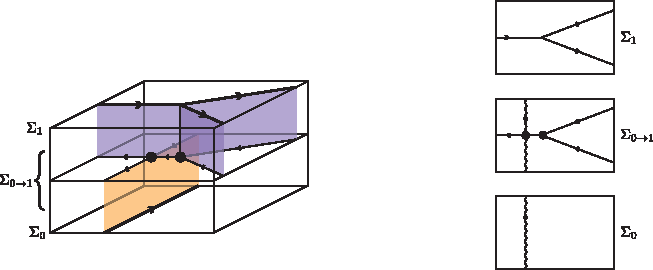
\includegraphics{CellDecomposition.pdf}
\caption{\label{CellDecomposition}
\dave{Will pitchforkize.} \ethan{Actually, I think it might be clearer if you don't. We mention the standardization procedure after we talk about the cell decomposition extension, and I think the figure is easier to look at pre-pitchforkization} 
The decomposition used to construct the shadow world tensor network, shown 
in its pre-standardized, pre-pitchforkization state.
The top layer $\Sigma_1$ is the cell decomposition that we use to construct the Hamiltonian in \eqref{ham}.
The bulk cell decomposition $\Sigma_{0\ra1}$ is found by extending $\Sigma_0$ into 
$\Sigma \times [0,\frac{1}{2}]$, and $\Sigma_{1}$ into $\Sigma \times [\frac{1}{2},1]$ (left figure).
The input cell decomposition $\Sigma_0$ is taken to be in `normal' position with respect to $\Sigma_1$, meaning that when each cell decomposition is extended into the bulk, the two decompositions only intersect transversely along edges. 
On the right, we have shown two dimensional representations of small patches of the cell decomposition. 
In the two dimensional pictures we will denote the cells stemming from $\Sigma_0$ by squiggly lines.
Notice that the orientation of all lines on $\Sigma_{0 \ra1}$ have been reversed relative to $\Sigma_0$ and $\Sigma_1$. 
}
\end{center}
\end{figure}

In order to evaluate $Z(\Sigma_{0\ra1}; v_0, v_1)$, we need to specify a cell decomposition on $\Sigma_{0\ra 1}$ (although the actual partition function is independent of the particular choice). 
We can take the cell decomposition in the bulk of $\Sigma_{0\ra1}$ to be any cell decomposition that agrees with the cell decomposition of $\Sigma_0$ and $\Sigma_1$ when restricted to $\partial \Sigma_{0\ra1}$.
However, there is a particularly convenient choice, which corresponds to extending the cell decomposition of $\Sigma_0$ into $\Sigma \times [0, 1/2]$, and that of $\Sigma_1$ into $\Sigma \times [1/2, 1]$, see Figure~\ref{CellDecomposition}. 
When we do this extension, every $k$-cell in $\Sigma_0$ and $\Sigma_1$ is extended into a $(k+1)$-cell in the bulk 
of $\Sigma_{0\ra1}$ (the $(k+1)$-cells are the `shadows' of the $k$-cells, and hence the bulk constitutes the `shadow world'\dave{never made that connection before, is that why they called it the shadow world?}
\kw{No, I don't think that's a correct etymology for ``shadow world".}). 
It is convenient to take the two cell decompositions on $\Sigma_0$ and $\Sigma_1$ to be in `normal' position,
meaning that the extension of $\Sigma_0$ into the bulk only intersects the extension of $\Sigma_1$ transversely along edges, again see Figure~\ref{CellDecomposition}.


We now specify the amplitude $Z(\Sigma_{0\ra 1}; v_0, v_1) $ in \eqref{GroundState}.
The amplitude is determined using the state sum procedure developed previously, and as such we will be brief in what follows. 
The labels of the 2-cells that extend from $\Sigma_0$ and $\Sigma_1$ are determined by $v_0$ and 
$v_1$, since they are the shadows of 1-cells in $\Sigma_0$ and $\Sigma_1$. 
The 2-cell labels living at $\Sigma \times \{ 1/2 \}$ are not fixed as input data however, and need to be 
summed over.
\dave{Should probably conform with notation in previous section}

As was done in our treatment of the state sum, to construct the weights ${\rm Link}(v,\beta)$ for a given 0-cell $v$ in $\Sigma \times \{1/2\}$, we insert a small $S^2$ around 
$v$ and examine the intersections of neighboring 2-cells with the $S^2$. These intersections 
are marked on the $S^2$ as edges, and the ${\rm Link}(v,\beta)$ are formed by evaluating 
the picture formed by these edges. 
\dave{Do we need to describe what $\text{Link}(v,\beta)$ is?}

\begin{figure}
\begin{center}
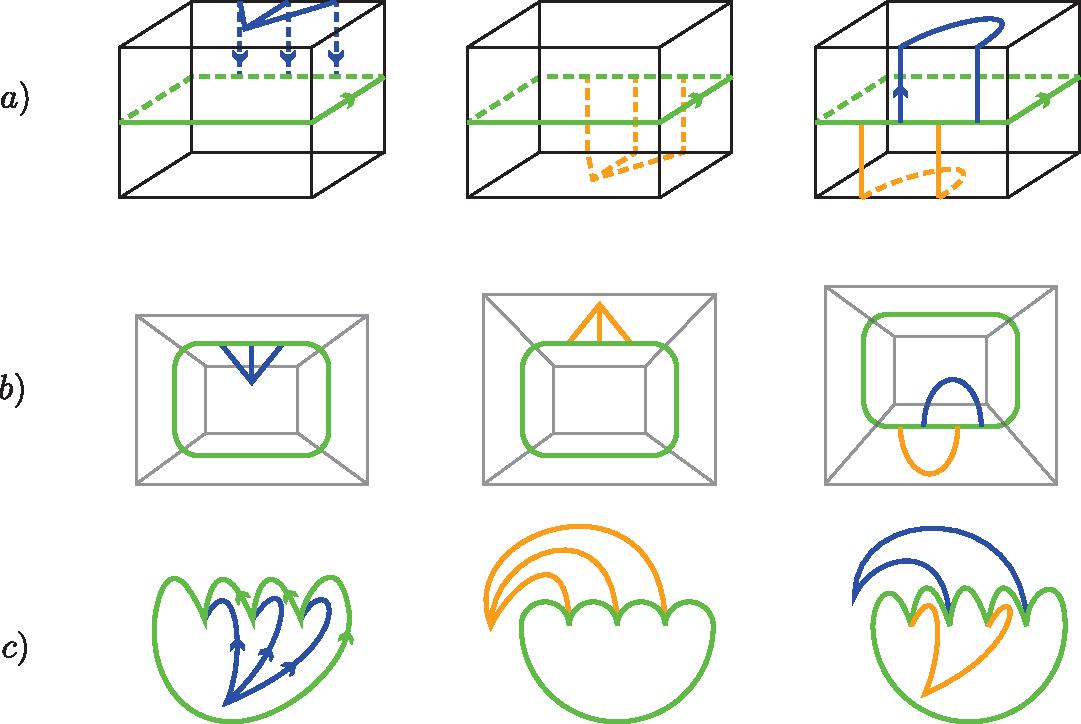
\includegraphics[scale=0.6]{StandardizedSlabTensors.pdf}
\caption{\label{StandardizedSlabTensors}
In row a) we show the three kinds of possible 0-cell tensors that could appear in the tensor contraction when 
computing the partition function $Z(\Sigma;v_0,v_1)$. The cube is drawn so that the 0-cell is located in the cube center. 
Blue (orange) lines represent intersections of 2-cells in the extension of the cell decomposition $\Sigma_1$ ($\Sigma_0$) with the cube, and 
green lines represent intersections of 2-cells in $\Sigma \times \{1/2\}$ with the cube. 
In row b) we show the first step for one possible standardization procedure, where the diagrams 
have been drawn projected into two dimensions. 
In row c) we finish the standardization of the diagrams by making each trivalent vertex a pitchfork. The appropriate 0-cell 
tensors are found by evaluation of these diagrams. 
}
\end{center}
\end{figure}

By looking at Figure~\ref{CellDecomposition}, we see that there are only three kinds of 0-cells that show up in 
$\Sigma \times \{1/2\}$: those that are formed at the x-shaped intersection of a 1-cell in the extension of $
\Sigma_0$ with a 1-cell in the extension of $\Sigma_1$, those where a 0-cell in the extension of $\Sigma_0$ 
meets the interior of a 2-cell in 
the extension of $\Sigma_1$, and vice versa. These possibilities lead to three different types of 0-cell weights that need to be evaluated. 
These three possibilities are illustrated in the top row $a)$ of Figure \ref{StandardizedSlabTensors}, where we have drawn a cube surrounding the 0-cell instead of an $S^2$.
In the figure, the blue (orange) lines denote 
the intersections of 2-cells in $\Sigma \times (1/2,1]$ (in $\Sigma \times [0,1/2)$) with the cube, 
and the green lines denote the intersection of 2-cells in $\Sigma \times \{1/2\}$ with the cube. 
The orientation of the lines drawn in these figures is fixed by the orientations of each of the 2-cells, 
which are determined with the aid of the orientation of $\Sigma$. 
In order to facilitate computations, we will need to standardize these diagrams according to the 
usual `pitchforkization' procedure employed in the previous sections. 
To do the standardization, we first project the diagrams into the plane (shown in the second row 
of Figure \ref{StandardizedSlabTensors}), and then deform each of the trivalent vertices 
to pitchforks. The final standardized diagrams are displayed in the third row of Figure \ref{StandardizedSlabTensors}.

The evaluation of these standardized diagrams gives the weight appearing in the partition function. 
Explicitly, for a 0-cell $v$ involving three neighboring 2-cells from the extension of $\Sigma_1$ (left column of row $a)$ in Figure \ref{StandardizedSlabTensors}, we assign the weight ${\rm Link}(v,\beta)$ as follows:
\begin{align}
\Tensora \; \ra {\rm Link}(v,\beta) &= \;  \Tensoraa %\cdot \mu_0 \tp s_1 \tp s_2 \tp s_3.
\end{align}
where $\beta$ denotes the labels provided by the indices $\mu_0,s_1, s_2, s_3$.

In the diagrams, the green letters $A,B,C$ denote the labels of the 2-cells in $\Sigma \times \{1/2\}$, which will 
be summed over when computing the amplitude $Z(\Sigma_{0\ra1}; v_0, v_1)$. The labels of 
the blue lines are fixed however, and determined by the labels of the 2-cells which are shadows of 1-cells 
in $\Sigma_1$. 

Weights for the other types of 0-cells in $\Sigma \times \{1/2\}$ are determined similarly. For the type of 
0-cell in the center column of row $a)$ in Figure \ref{StandardizedSlabTensors}, we assign the weight
\begin{align}
\Tensorc \;\ra {\rm Link}(v,\beta) &= \; \Tensorcc % \cdot \nu_0 \tp s_1 \tp s_2 \tp s_3, \\
\end{align}
while for the type of 0-cell in the last column we assign the weight
\begin{align}
\Tensorb \; \ra {\rm Link}(v,\beta) &= \;  \Tensorbb  %\cdot s_0 \tp s_1 \tp s_2 \tp s_3, \\
\end{align}
which corresponds to a string operator. 
%In all of these weig, we are making use of the implicit left-to-right Koszul ordering convention for the 
%tensor factors. 
\dave{I think we should write these as tensors. 
We should also specify which vertices pick up a $(-1)^{|\mu|}$.} 

In order to perform the contraction that will compute the partition function, all the 1-cells 
$\Sigma \times \{1/2\}$ need an orientation. Since these 1-cells biject with the 1-cells of $\Sigma_0$ and $\Sigma_1$ (they are all shadows of 1-cells in either $\Sigma_0$ or $\Sigma_1$ from our 
choice of cell decomposition in $\Sigma_{0\ra1}$), we can assign an orientation to each 1-handle in 
$\Sigma \times \{1/2\}$ using the orientation of the 1-cells in $\Sigma_0$ and $\Sigma_1$, which 
are fixed by the states $v_0$ and $v_1$.

We can now compute $Z(\Sigma_{0\ra1}; v_0, v_1)$ 
using the state sum: 
\begin{align} 
Z(\Sigma_{0\ra1}; v_0, v_1) = \sum_{ \beta\in\mcl(\mch^{1/2})_{bulk}}  (-1)^{\kappa_\beta} \prod_{f \in \mch^{1/2}_2} \frac{d(f,\beta)}{n(f,\beta)} 
\prod_{e \in \mch^{1/2}_1} \widetilde{\Theta}(P_e,\beta)^{-1} \prod_{v \in \mch^{1/2}_0} {\rm Link}(v,\beta),
\end{align} 
where we have used $\mch^{1/2}_k$ to denote the collection of $k$-cells in $\Sigma \times \{1/2\}$ and $\mcl(\mch^{1/2})_{bulk}$ 
to denote colorings of the bulk degrees of freedom in $\Sigma_{0\ra1}$. 


